% ============================================================================
% BÁO CÁO MÔN HỌC: CƠ SỞ DỮ LIỆU TIÊN TIẾN
% Đề tài: Xây dựng hệ thống e-Library phân tán nhiều cơ sở
% Nhóm 10 - Cao học K35
% Trường Đại học Sư phạm Hà Nội
% ============================================================================
\documentclass[a4paper,12pt]{report}

% ============================================================================
% PACKAGES
% ============================================================================
\usepackage[utf8]{inputenc}
\usepackage[T5]{fontenc}
\usepackage[vietnamese]{babel}
\usepackage[top=2.5cm, bottom=2.5cm, left=3cm, right=2cm]{geometry}
\usepackage{graphicx}
\usepackage{listings}
\usepackage{xcolor}
\usepackage{hyperref}
\usepackage{fancyhdr}
\usepackage{tikz}
\usepackage{booktabs}
\usepackage{longtable}
\usepackage{float}
\usepackage{indentfirst}
\usepackage{caption}
\usepackage{subcaption}
\usepackage{amsmath}
\usepackage{amssymb}
\usepackage{enumitem}
\usepackage{array}
\usepackage{tabularx}
\usepackage{multirow}

% ============================================================================
% TikZ Libraries
% ============================================================================
\usetikzlibrary{shapes.geometric, arrows, positioning, fit, backgrounds, calc}

% ============================================================================
% Hyperref Configuration
% ============================================================================
\hypersetup{
    colorlinks=true,
    linkcolor=blue,
    filecolor=magenta,
    urlcolor=cyan,
    pdftitle={e-Library Distributed System - Hệ thống thư viện phân tán},
    pdfauthor={Nhom 10 - Cao hoc K35 - HNUE},
    pdfsubject={Cơ sở dữ liệu tiên tiến},
    pdfkeywords={MongoDB, Distributed Systems, NoSQL, PHP, Docker}
}

% ============================================================================
% Listings Configuration (for code)
% ============================================================================
\definecolor{codegreen}{rgb}{0,0.6,0}
\definecolor{codegray}{rgb}{0.5,0.5,0.5}
\definecolor{codepurple}{rgb}{0.58,0,0.82}
\definecolor{backcolour}{rgb}{0.95,0.95,0.92}
\definecolor{keywordcolor}{rgb}{0.0,0.0,0.6}
\definecolor{stringcolor}{rgb}{0.6,0.1,0.1}

\lstdefinestyle{mystyle}{
    backgroundcolor=\color{backcolour},
    commentstyle=\color{codegreen},
    keywordstyle=\color{keywordcolor}\bfseries,
    numberstyle=\tiny\color{codegray},
    stringstyle=\color{stringcolor},
    basicstyle=\ttfamily\footnotesize,
    breakatwhitespace=false,
    breaklines=true,
    captionpos=b,
    keepspaces=true,
    numbers=left,
    numbersep=5pt,
    showspaces=false,
    showstringspaces=false,
    showtabs=false,
    tabsize=2,
    frame=single,
    framesep=3pt,
    xleftmargin=15pt,
    xrightmargin=5pt,
}

\lstset{style=mystyle}

% Define PHP language for listings
\lstdefinelanguage{PHP}{
    keywords={class, function, return, if, else, elseif, foreach, for, while, do, switch, case, break, continue, echo, print, require, require_once, include, include_once, new, public, private, protected, static, const, var, true, false, null, array, try, catch, throw, use, namespace},
    sensitive=true,
    morecomment=[l]{//},
    morecomment=[s]{/*}{*/},
    morestring=[b]",
    morestring=[b]',
}

% Define JSON language
\lstdefinelanguage{json}{
    morestring=[b]",
    morestring=[b]',
    literate=
     *{0}{{{\color{codepurple}0}}}{1}
      {1}{{{\color{codepurple}1}}}{1}
      {2}{{{\color{codepurple}2}}}{1}
      {3}{{{\color{codepurple}3}}}{1}
      {4}{{{\color{codepurple}4}}}{1}
      {5}{{{\color{codepurple}5}}}{1}
      {6}{{{\color{codepurple}6}}}{1}
      {7}{{{\color{codepurple}7}}}{1}
      {8}{{{\color{codepurple}8}}}{1}
      {9}{{{\color{codepurple}9}}}{1}
      {:}{{{\color{red}:}}}{1}
      {,}{{{\color{red},}}}{1}
      {\{}{{{\color{blue}\{}}}{1}
      {\}}{{{\color{blue}\}}}}{1}
      {[}{{{\color{blue}[}}}{1}
      {]}{{{\color{blue}]}}}{1},
}

% Define YAML language
\lstdefinelanguage{yaml}{
    keywords={true, false, null},
    sensitive=false,
    morecomment=[l]{\#},
    morestring=[b]",
    morestring=[b]',
}

% Define JavaScript language
\lstdefinelanguage{javascript}{
    keywords={break, case, catch, continue, debugger, default, delete, do, else, finally, for, function, if, in, instanceof, new, return, switch, this, throw, try, typeof, var, void, while, with, let, const, class, export, extends, import, super, yield, async, await},
    sensitive=true,
    morecomment=[l]{//},
    morecomment=[s]{/*}{*/},
    morestring=[b]",
    morestring=[b]',
    morestring=[b]`,
}

% ============================================================================
% Header/Footer Configuration
% ============================================================================
\pagestyle{fancy}
\fancyhf{}
\fancyhead[L]{\leftmark}
\fancyhead[R]{e-Library Distributed System}
\fancyfoot[C]{\thepage}
\renewcommand{\headrulewidth}{0.4pt}
\renewcommand{\footrulewidth}{0.4pt}

% Clear header/footer for chapter pages
\fancypagestyle{plain}{
    \fancyhf{}
    \fancyfoot[C]{\thepage}
    \renewcommand{\headrulewidth}{0pt}
    \renewcommand{\footrulewidth}{0.4pt}
}

% ============================================================================
% Graphics Path
% ============================================================================
\graphicspath{{screenshots/}{figures/}{../screenshots/}}

% ============================================================================
% Custom Commands
% ============================================================================
\newcommand{\code}[1]{\texttt{#1}}
\newcommand{\mongodb}{\texttt{MongoDB}}
\newcommand{\php}{\texttt{PHP}}
\newcommand{\docker}{\texttt{Docker}}

% Centered table column with fixed width
\newcolumntype{C}[1]{>{\centering\arraybackslash}p{#1}}
\newcolumntype{L}[1]{>{\raggedright\arraybackslash}p{#1}}
\newcolumntype{R}[1]{>{\raggedleft\arraybackslash}p{#1}}

% ============================================================================
% Document Information
% ============================================================================
\title{
    \textbf{BÁO CÁO MÔN HỌC} \\
    \textbf{CƠ SỞ DỮ LIỆU TIÊN TIẾN} \\
    \vspace{1cm}
    \large Đề tài: Xây dựng hệ thống e-Library phân tán nhiều cơ sở \\
    với MongoDB Replica Set
}
\author{
    Nhóm 10 - Cao học K35 \\
    Trường Đại học Sư phạm Hà Nội
}
\date{Tháng 1, 2026}

% ============================================================================
% DOCUMENT
% ============================================================================
\begin{document}

% Title page
% ============================================================================
% TRANG BÌA
% ============================================================================
\begin{titlepage}
\begin{center}

% Logo trường (nếu có)
% \includegraphics[width=3cm]{figures/hnue_logo.png}\\[0.5cm]

\textbf{\Large TRƯỜNG ĐẠI HỌC SƯ PHẠM HÀ NỘI}\\[0.3cm]
\textbf{\large KHOA CÔNG NGHỆ THÔNG TIN}\\[1.5cm]

% Tên môn học
\textbf{\Large BÁO CÁO MÔN HỌC}\\[0.3cm]
\textbf{\LARGE CƠ SỞ DỮ LIỆU TIÊN TIẾN}\\[1cm]

% Đường kẻ
\rule{\textwidth}{0.5pt}\\[0.5cm]

% Tên đề tài
{\huge \textbf{XÂY DỰNG HỆ THỐNG E-LIBRARY}}\\[0.3cm]
{\huge \textbf{PHÂN TÁN NHIỀU CƠ SỞ}}\\[0.5cm]

\rule{\textwidth}{0.5pt}\\[1.5cm]

% Thông tin nhóm
\begin{minipage}[t]{0.45\textwidth}
\begin{flushleft}
\textbf{\large Giảng viên hướng dẫn:}\\[0.3cm]
TS. Nguyễn Duy Hải
\end{flushleft}
\end{minipage}
\hfill
\begin{minipage}[t]{0.45\textwidth}
\begin{flushright}
\textbf{\large Nhóm thực hiện:}\\[0.3cm]
Nhóm 10 - Cao học K35\\[0.5cm]
\textbf{Thành viên:}\\[0.2cm]
1. Trương Tuấn Nghĩa\\
2. Phạm Mạnh Thắng\\
3. Lưu Anh Tú\\[0.5cm]
\textbf{Liên hệ:}\\[0.1cm]
\small truongtuannghia1248@gmail.com\\
\small 0973 958 574
\end{flushright}
\end{minipage}

\vfill

% Công nghệ sử dụng
\begin{center}
\textbf{Công nghệ:} MongoDB 8.0 | PHP 8.4 | Docker | Chart.js
\end{center}

\vspace{0.5cm}

% GitHub Repository
\begin{center}
\fbox{\parbox{0.8\textwidth}{
\centering
\textbf{Mã nguồn dự án (GitHub):}\\[0.2cm]
\url{https://github.com/TatcataiTTN/Final-CSDLTT-HNUE-distributed-elibrary}\\[0.2cm]
\small \textit{Hướng dẫn cài đặt chi tiết có trong file README của repository}
}}
\end{center}

\vspace{0.5cm}

% Năm học
\textbf{\large Hà Nội, tháng 01 năm 2026}

\end{center}
\end{titlepage}


% Front matter
\pagenumbering{roman}

% Lời cảm ơn
% ============================================================================
% LỜI CẢM ƠN
% ============================================================================
\chapter*{LỜI CẢM ƠN}
\addcontentsline{toc}{chapter}{LỜI CẢM ƠN}

Lời đầu tiên, nhóm chúng em xin gửi lời cảm ơn chân thành và sâu sắc nhất đến \textbf{TS. Nguyễn Duy Hải} - giảng viên hướng dẫn môn Cơ sở dữ liệu tiên tiến. Thầy đã tận tình giảng dạy, truyền đạt những kiến thức quý báu về hệ thống cơ sở dữ liệu phân tán và NoSQL, đồng thời hướng dẫn nhóm trong suốt quá trình thực hiện đề tài.

Chúng em xin cảm ơn \textbf{Khoa Công nghệ Thông tin - Trường Đại học Sư phạm Hà Nội} đã tạo điều kiện thuận lợi về cơ sở vật chất và môi trường học tập để nhóm có thể hoàn thành tốt bài báo cáo này.

Chúng em cũng xin gửi lời cảm ơn đến các bạn học viên lớp Cao học K35 đã chia sẻ kinh nghiệm và hỗ trợ nhóm trong quá trình học tập và nghiên cứu.

Do thời gian và kiến thức còn hạn chế, bài báo cáo không tránh khỏi những thiếu sót. Nhóm chúng em rất mong nhận được sự góp ý, chỉ bảo của Thầy và các bạn để bài báo cáo được hoàn thiện hơn.

Xin chân thành cảm ơn!

\vspace{1cm}
\begin{flushright}
\textit{Hà Nội, tháng 01 năm 2026}\\[0.5cm]
\textbf{Nhóm thực hiện}\\[0.3cm]
Trương Tuấn Nghĩa\\
Phạm Mạnh Thắng\\
Lưu Anh Tú
\end{flushright}


% Lời cam đoan
% ============================================================================
% LỜI CAM ĐOAN
% ============================================================================
\chapter*{LỜI CAM ĐOAN}
\addcontentsline{toc}{chapter}{LỜI CAM ĐOAN}

Chúng tôi xin cam đoan:

\begin{enumerate}
    \item Đề tài báo cáo môn học \textbf{"Xây dựng hệ thống e-Library phân tán nhiều cơ sở"} là công trình nghiên cứu và thực hiện của nhóm chúng tôi dưới sự hướng dẫn của \textbf{TS. Nguyễn Duy Hải}.

    \item Các số liệu, kết quả benchmark và kịch bản kiểm thử trong báo cáo là trung thực và được thực hiện trên hệ thống thực tế.

    \item Mã nguồn được phát triển bởi nhóm, có tham khảo và sử dụng các thư viện mã nguồn mở theo đúng quy định (MongoDB PHP Library, Firebase PHP-JWT, Chart.js).

    \item Các tài liệu tham khảo được trích dẫn đầy đủ theo quy định.
\end{enumerate}

Chúng tôi xin chịu hoàn toàn trách nhiệm về lời cam đoan này.

\vspace{1.5cm}
\begin{flushright}
\textit{Hà Nội, ngày \hspace{0.5cm} tháng 01 năm 2026}\\[0.8cm]
\textbf{Nhóm thực hiện}\\[1cm]
\textbf{Trương Tuấn Nghĩa}\\[0.3cm]
\textbf{Phạm Mạnh Thắng}\\[0.3cm]
\textbf{Lưu Anh Tú}
\end{flushright}


% Mục lục
\tableofcontents
\newpage

% Danh mục hình
\listoffigures
\addcontentsline{toc}{chapter}{DANH MỤC HÌNH}
\newpage

% Danh mục bảng
\listoftables
\addcontentsline{toc}{chapter}{DANH MỤC BẢNG}
\newpage

% Danh mục mã nguồn
\lstlistoflistings
\addcontentsline{toc}{chapter}{DANH MỤC MÃ NGUỒN}
\newpage

% ============================================================================
% MAIN MATTER
% ============================================================================
\pagenumbering{arabic}

% Chương I & II: Tổng quan và Phân tích thiết kế
% ============================================================================
% CHƯƠNG I: TỔNG QUAN VỀ HỆ THỐNG
% ============================================================================
\chapter{TỔNG QUAN VỀ HỆ THỐNG}

\section{Giới thiệu bài toán và mục tiêu hệ thống}

\subsection{Bối cảnh và đặt vấn đề}

Trong bối cảnh số hóa và phát triển công nghệ thông tin, các thư viện truyền thống đang dần chuyển đổi sang mô hình thư viện điện tử (e-Library). Đối với các hệ thống thư viện có nhiều chi nhánh phân bố ở các vị trí địa lý khác nhau, việc quản lý tập trung và đồng bộ dữ liệu trở thành một thách thức lớn.

Các vấn đề cần giải quyết:
\begin{itemize}
    \item \textbf{Tính phân tán}: Dữ liệu cần được lưu trữ và truy cập từ nhiều vị trí địa lý khác nhau
    \item \textbf{Tính sẵn sàng cao}: Hệ thống phải hoạt động liên tục, có khả năng tự phục hồi khi gặp sự cố
    \item \textbf{Hiệu năng}: Đảm bảo thời gian phản hồi nhanh cho các truy vấn dữ liệu
    \item \textbf{Khả năng mở rộng}: Hệ thống có thể scale theo chiều ngang khi lượng dữ liệu tăng
\end{itemize}

\subsection{Mục tiêu của đề tài}

Đề tài \textbf{"Xây dựng hệ thống E-Library Phân tán nhiều cơ sở"} hướng đến các mục tiêu sau:

\begin{enumerate}
    \item \textbf{Thiết kế và cài đặt hệ thống phân tán}:
    \begin{itemize}
        \item Kiến trúc 4 node: 1 Central Hub + 3 chi nhánh (Hà Nội, Đà Nẵng, TP.HCM)
        \item Sử dụng MongoDB Replica Set cho high availability
        \item Hỗ trợ Zone Sharding theo vùng địa lý
    \end{itemize}

    \item \textbf{Triển khai các kỹ thuật NoSQL nâng cao}:
    \begin{itemize}
        \item Aggregation Pipeline với 10+ operators
        \item Map-Reduce cho phân tích dữ liệu phức tạp
        \item Full-text Search với TEXT index
    \end{itemize}

    \item \textbf{Đảm bảo bảo mật và phân quyền}:
    \begin{itemize}
        \item JWT (JSON Web Token) authentication
        \item Role-based Access Control (RBAC)
        \item Password hashing với bcrypt
    \end{itemize}

    \item \textbf{Xây dựng giao diện quản trị}:
    \begin{itemize}
        \item Dashboard thống kê với Chart.js
        \item CRUD đầy đủ cho sách, người dùng, đơn hàng
        \item Responsive design với Bootstrap 5
    \end{itemize}
\end{enumerate}

\section{Tổng quan về hệ thống e-Library}

\subsection{Mô hình hệ thống phân tán}

Hệ thống e-Library được thiết kế theo mô hình phân tán với 4 node độc lập, mỗi node có database riêng nhưng được đồng bộ qua MongoDB Replica Set:

\begin{table}[H]
\centering
\caption{Các node trong hệ thống e-Library}
\label{tab:nodes}
\begin{tabular}{|c|l|l|c|l|}
\hline
\textbf{STT} & \textbf{Node} & \textbf{Database} & \textbf{Port} & \textbf{Vai trò} \\
\hline
1 & Central Hub & Nhasach & 8001 & Trung tâm quản lý \\
2 & Branch Hà Nội & NhasachHaNoi & 8002 & Chi nhánh miền Bắc \\
3 & Branch Đà Nẵng & NhasachDaNang & 8003 & Chi nhánh miền Trung \\
4 & Branch TP.HCM & NhasachHoChiMinh & 8004 & Chi nhánh miền Nam \\
\hline
\end{tabular}
\end{table}

\subsection{Dữ liệu thực tế trong hệ thống}

Tính đến thời điểm hoàn thành đề tài, hệ thống có các số liệu sau:

\begin{table}[H]
\centering
\caption{Thống kê dữ liệu theo từng chi nhánh}
\label{tab:data_stats}
\begin{tabular}{|l|r|r|r|}
\hline
\textbf{Chi nhánh} & \textbf{Số sách} & \textbf{Số users} & \textbf{Số orders} \\
\hline
Central Hub (Nhasach) & 509 & 42 & 111 \\
Chi nhánh Hà Nội & 200 & 13 & 46 \\
Chi nhánh Đà Nẵng & 163 & 12 & 16 \\
Chi nhánh TP.HCM & 146 & 11 & 14 \\
\hline
\textbf{Tổng cộng} & \textbf{1.018} & \textbf{78} & \textbf{187} \\
\hline
\end{tabular}
\end{table}

\subsection{Kiến trúc tổng quan}

\begin{figure}[H]
\centering
\begin{tikzpicture}[
    node distance=1.5cm,
    box/.style={rectangle, draw, rounded corners, minimum width=3.2cm, minimum height=1.1cm, align=center, font=\small},
    db/.style={cylinder, draw, shape border rotate=90, minimum width=2cm, minimum height=1.2cm, aspect=0.25, font=\scriptsize, align=center},
    arrow/.style={->, >=stealth, thick}
]
    % Client Layer
    \node[box, fill=blue!15, drop shadow] (client) at (0,6) {\textbf{Web Browser}\\Admin/Customer};

    % PHP Application Layer - Central Hub
    \node[box, fill=green!25, drop shadow] (central) at (0,4) {\textbf{Central Hub}\\PHP 8.4 | Port 8001\\DB: Nhasach};

    % PHP Application Layer - Branches
    \node[box, fill=green!15] (hanoi) at (-5,2) {\textbf{Chi nhánh HN}\\Port 8002\\DB: NhasachHaNoi};
    \node[box, fill=green!15] (danang) at (0,2) {\textbf{Chi nhánh ĐN}\\Port 8003\\DB: NhasachDaNang};
    \node[box, fill=green!15] (hcm) at (5,2) {\textbf{Chi nhánh HCM}\\Port 8004\\DB: NhasachHoChiMinh};

    % MongoDB Layer - 4 separate databases
    \node[db, fill=orange!20] (mongo1) at (-5,0) {MongoDB\\mongo1\\:27017\\Nhasach};
    \node[db, fill=orange!15] (mongo2) at (-1.5,0) {MongoDB\\mongo2\\:27018\\NhasachHaNoi};
    \node[db, fill=orange!15] (mongo3) at (1.5,0) {MongoDB\\mongo3\\:27019\\NhasachDaNang};
    \node[db, fill=orange!15] (mongo4) at (5,0) {MongoDB\\mongo4\\:27020\\NhasachHoChiMinh};

    % Connections - Client to Central
    \draw[arrow, blue, line width=1.2pt] (client) -- (central);

    % Connections - Central to Branches (sync)
    \draw[arrow, red, dashed, line width=1pt] (central) -- node[left, font=\tiny] {sync} (hanoi);
    \draw[arrow, red, dashed, line width=1pt] (central) -- node[right, font=\tiny] {sync} (danang);
    \draw[arrow, red, dashed, line width=1pt] (central) -- node[right, font=\tiny] {sync} (hcm);

    % Connections - PHP to MongoDB
    \draw[arrow, green!60!black, line width=1pt] (central) -- (mongo1);
    \draw[arrow, green!60!black, line width=1pt] (hanoi) -- (mongo2);
    \draw[arrow, green!60!black, line width=1pt] (danang) -- (mongo3);
    \draw[arrow, green!60!black, line width=1pt] (hcm) -- (mongo4);

    % Labels
    \node[font=\tiny, text=gray] at (0,-1.2) {Mỗi chi nhánh có database MongoDB riêng biệt};

\end{tikzpicture}
\caption{Kiến trúc tổng quan hệ thống e-Library phân tán 4 cơ sở}
\label{fig:architecture}
\end{figure}

\section{Một số khái niệm và nghiệp vụ liên quan}

\subsection{Khái niệm về các đối tượng}

\begin{enumerate}
    \item \textbf{Quản trị viên hệ thống (Admin)}:
    \begin{itemize}
        \item Toàn quyền quản lý hệ thống tại Central Hub
        \item Quản lý sách, người dùng, đơn hàng
        \item Xem Dashboard thống kê
        \item Đồng bộ dữ liệu giữa các chi nhánh
    \end{itemize}

    \item \textbf{Quản trị viên chi nhánh (Branch Admin)}:
    \begin{itemize}
        \item Quản lý sách tại chi nhánh được phân công
        \item Username: adminHN, adminDN, adminHCM
        \item Không thể can thiệp vào chi nhánh khác
    \end{itemize}

    \item \textbf{Khách hàng (Customer)}:
    \begin{itemize}
        \item Đăng ký tài khoản tại chi nhánh
        \item Tìm kiếm, xem thông tin sách
        \item Mượn sách qua giỏ hàng
        \item Xem lịch sử mượn sách
    \end{itemize}
\end{enumerate}

\subsection{Các quy trình nghiệp vụ}

\begin{enumerate}
    \item \textbf{Quy trình đăng ký/đăng nhập}:
    \begin{itemize}
        \item Khách hàng đăng ký với username, password, email
        \item Mật khẩu được hash bằng bcrypt (cost factor 12)
        \item Đăng nhập tạo JWT token với thời hạn 24 giờ
        \item Token được lưu trong session hoặc Authorization header
    \end{itemize}

    \item \textbf{Quy trình tìm kiếm sách}:
    \begin{itemize}
        \item Hỗ trợ Full-text Search với TEXT index
        \item Tìm theo tên sách, thể loại, tác giả
        \item Kết quả được sắp xếp theo relevance score
        \item Hỗ trợ phân trang với 20 sách/trang
    \end{itemize}

    \item \textbf{Quy trình mượn sách}:
    \begin{itemize}
        \item Khách hàng thêm sách vào giỏ hàng
        \item Chọn số ngày mượn, hệ thống tính tiền
        \item Xác nhận đơn mượn, trừ số dư
        \item Trạng thái đơn: pending $\rightarrow$ paid $\rightarrow$ success $\rightarrow$ returned
    \end{itemize}

    \item \textbf{Quy trình đồng bộ dữ liệu}:
    \begin{itemize}
        \item Chi nhánh gửi dữ liệu về Central Hub qua REST API
        \item Sử dụng script \texttt{sync\_data.sh} để đồng bộ
        \item Dữ liệu customers và orders được tổng hợp tại Central
    \end{itemize}
\end{enumerate}

\section{Một số công nghệ được áp dụng}

\subsection{PHP 8.4 và MongoDB Driver}

PHP (Hypertext Preprocessor) là ngôn ngữ lập trình kịch bản phía server, được sử dụng rộng rãi trong phát triển ứng dụng web. Trong đề tài này, nhóm sử dụng \textbf{PHP 8.4} kết hợp với thư viện \texttt{mongodb/mongodb v2.1}.

\textbf{Đặc điểm của mongodb/mongodb library}:
\begin{itemize}
    \item Hỗ trợ đầy đủ CRUD operations với type-safe API
    \item Aggregation Pipeline Builder cho truy vấn phức tạp
    \item Hỗ trợ BSON types (ObjectId, UTCDateTime, Javascript)
    \item Connection pooling tự động
    \item Read/Write Concern configuration
\end{itemize}

\textbf{Cấu hình kết nối trong Connection.php}:

File \texttt{Connection.php} là điểm trung tâm quản lý kết nối đến MongoDB cho toàn bộ ứng dụng. File này hỗ trợ 3 chế độ kết nối: \textbf{standalone} (một máy chủ đơn), \textbf{replicaset} (cluster 3 nodes với failover tự động), và \textbf{sharded} (phân mảnh dữ liệu theo vùng). Tham số \texttt{readPreference: primaryPreferred} cho phép đọc từ Secondary nếu Primary quá tải, còn \texttt{w: majority} đảm bảo dữ liệu được ghi vào đa số nodes trước khi xác nhận thành công - đây là chiến lược cân bằng giữa hiệu năng và độ tin cậy.

\begin{lstlisting}[language=PHP, caption=Connection.php - Cấu hình kết nối MongoDB]
<?php
require 'vendor/autoload.php';
use MongoDB\Client;

$MODE = 'sharded'; // Options: standalone, replicaset, sharded
$Database = "Nhasach";

switch ($MODE) {
    case 'sharded':
        $conn = new Client("mongodb://localhost:27017", [
            'readPreference' => 'primaryPreferred',
            'w' => 'majority',
            'journal' => true
        ]);
        break;
    case 'replicaset':
        $conn = new Client(
            "mongodb://mongo1:27017,mongo2:27017,mongo3:27017/?replicaSet=rs0",
            ['readPreference' => 'primaryPreferred', 'w' => 'majority']
        );
        break;
    default:
        $conn = new Client("mongodb://localhost:27017");
}
$db = $conn->$Database;
\end{lstlisting}

\subsection{MongoDB và MongoDB Compass}

\textbf{MongoDB} là hệ quản trị cơ sở dữ liệu NoSQL hướng tài liệu (document-oriented), lưu trữ dữ liệu dưới dạng BSON (Binary JSON). Phiên bản sử dụng: \textbf{MongoDB 4.4} (Docker image).

\textbf{Các tính năng MongoDB được sử dụng trong đề tài}:
\begin{itemize}
    \item \textbf{Replica Set}: 3 nodes (mongo1, mongo2, mongo3) với automatic failover
    \item \textbf{Aggregation Pipeline}: 10+ operators (\$match, \$group, \$sort, \$lookup, \$facet, \$bucket...)
    \item \textbf{Map-Reduce}: 5 operations cho phân tích phức tạp
    \item \textbf{TEXT Index}: Full-text search tiếng Việt
    \item \textbf{Compound Index}: Tối ưu shard-aware queries
\end{itemize}

\textbf{MongoDB Compass} là công cụ GUI chính thức, hỗ trợ:
\begin{itemize}
    \item Trực quan hóa dữ liệu và cấu trúc schema
    \item Aggregation Pipeline Builder với drag-and-drop
    \item Explain Plan để phân tích query performance
    \item Real-time server statistics
\end{itemize}

\subsection{Docker và Docker Compose}

\textbf{Docker} là nền tảng container hóa cho phép đóng gói ứng dụng cùng dependencies. \textbf{Docker Compose} cho phép định nghĩa multi-container applications.

\textbf{Vai trò trong đề tài}:
\begin{itemize}
    \item Khởi tạo MongoDB Replica Set với 3 containers
    \item Mạng nội bộ \texttt{mongo-net} cho giao tiếp giữa các nodes
    \item Volume persistence cho dữ liệu (\texttt{mongo1\_data}, \texttt{mongo2\_data}, \texttt{mongo3\_data})
    \item Dễ dàng tái lập kịch bản Failover testing
\end{itemize}

Đoạn cấu hình Docker Compose dưới đây định nghĩa một MongoDB Replica Set gồm 3 containers: \texttt{mongo1} (Primary, cổng 27017), \texttt{mongo2} và \texttt{mongo3} (Secondary, cổng 27018 và 27019). Tham số \texttt{--replSet rs0} cho biết cả 3 containers thuộc cùng một replica set tên ``rs0''. Mạng \texttt{mongo-net} với driver \texttt{bridge} cho phép các containers giao tiếp nội bộ. Khi \texttt{mongo1} gặp sự cố, một trong hai Secondary sẽ tự động được bầu làm Primary mới trong vòng 10-12 giây.

\begin{lstlisting}[caption=docker-compose.yml - MongoDB Replica Set]
version: '3.8'
services:
  mongo1:
    image: mongo:4.4
    container_name: mongo1
    ports: ["27017:27017"]
    command: ["mongod", "--replSet", "rs0", "--bind_ip_all"]
    volumes: [mongo1_data:/data/db]
    networks: [mongo-net]

  mongo2:
    image: mongo:4.4
    ports: ["27018:27017"]
    command: ["mongod", "--replSet", "rs0", "--bind_ip_all"]
    depends_on: [mongo1]

  mongo3:
    image: mongo:4.4
    ports: ["27019:27017"]
    command: ["mongod", "--replSet", "rs0", "--bind_ip_all"]
    depends_on: [mongo1]

networks:
  mongo-net:
    driver: bridge
\end{lstlisting}

\subsection{JWT (JSON Web Token)}

JWT là chuẩn mở (RFC 7519) để truyền thông tin an toàn giữa các bên dưới dạng JSON object. Thư viện \texttt{firebase/php-jwt v6.x} được sử dụng.

\textbf{Cấu trúc JWT trong hệ thống}:
\begin{itemize}
    \item \textbf{Header}: Algorithm HS256
    \item \textbf{Payload}: user\_id, username, role, node\_id, iat, exp
    \item \textbf{Signature}: HMAC-SHA256 với secret key
\end{itemize}

\begin{lstlisting}[language=PHP, caption=JWTHelper.php - Tạo JWT Token]
public static function generateToken($userId, $username, $role, $nodeId = null) {
    $payload = [
        'iss' => JWT_ISSUER,
        'iat' => time(),
        'exp' => time() + (24 * 3600), // 24 hours
        'nbf' => time(),
        'data' => [
            'user_id'  => $userId,
            'username' => $username,
            'role'     => $role,
            'node_id'  => $nodeId ?? JWT_NODE_ID
        ]
    ];
    return JWT::encode($payload, JWT_SECRET_KEY, 'HS256');
}
\end{lstlisting}

\subsection{Chart.js}

Chart.js là thư viện JavaScript mã nguồn mở để vẽ biểu đồ. Phiên bản 4.4 được sử dụng cho Dashboard.

\textbf{Các loại biểu đồ được sử dụng}:
\begin{itemize}
    \item \textbf{Bar Chart}: Số lượng sách theo chi nhánh, top sách được mượn
    \item \textbf{Pie/Doughnut Chart}: Phân bố người dùng theo role, trạng thái đơn hàng
    \item \textbf{Line Chart}: Xu hướng mượn sách theo thời gian
\end{itemize}

% ============================================================================
% CHƯƠNG II: PHÂN TÍCH VÀ THIẾT KẾ HỆ THỐNG
% ============================================================================
\chapter{PHÂN TÍCH VÀ THIẾT KẾ HỆ THỐNG}

\section{Xác định các yêu cầu}

\subsection{Yêu cầu phi chức năng}

\begin{enumerate}
    \item \textbf{Tính sẵn sàng cao (High Availability)}:
    \begin{itemize}
        \item Hệ thống hoạt động 24/7
        \item Tự động failover khi 1/3 nodes gặp sự cố
        \item Recovery time: 10-15 giây
    \end{itemize}

    \item \textbf{Hiệu năng (Performance)}:
    \begin{itemize}
        \item Thời gian phản hồi trung bình < 3ms
        \item Throughput: 500+ ops/sec
        \item Hỗ trợ concurrent users
    \end{itemize}

    \item \textbf{Khả năng mở rộng (Scalability)}:
    \begin{itemize}
        \item Horizontal scaling: thêm shard không cần downtime
        \item Zone-based sharding theo địa lý
    \end{itemize}

    \item \textbf{Bảo mật (Security)}:
    \begin{itemize}
        \item JWT authentication với expiration
        \item bcrypt password hashing (cost 12)
        \item RBAC: admin/customer roles
        \item Brute-force protection
    \end{itemize}

    \item \textbf{Nhất quán dữ liệu (Consistency)}:
    \begin{itemize}
        \item Write Concern: majority
        \item Read Preference: primaryPreferred
        \item Replication lag < 500ms
    \end{itemize}
\end{enumerate}

\subsection{Yêu cầu chức năng}

\begin{table}[H]
\centering
\caption{Danh sách yêu cầu chức năng}
\label{tab:functional_req}
\begin{tabular}{|c|l|l|l|}
\hline
\textbf{STT} & \textbf{Chức năng} & \textbf{Actor} & \textbf{Mô tả} \\
\hline
1 & Đăng ký tài khoản & Customer & Tạo account mới \\
2 & Đăng nhập/Đăng xuất & All & JWT authentication \\
3 & Quản lý sách (CRUD) & Admin & Thêm/Sửa/Xóa sách \\
4 & Tìm kiếm sách & All & Full-text search \\
5 & Quản lý người dùng & Admin & CRUD users \\
6 & Giỏ hàng & Customer & Thêm/Xóa sách \\
7 & Đặt mượn sách & Customer & Tạo đơn mượn \\
8 & Lịch sử mượn & Customer & Xem orders \\
9 & Dashboard thống kê & Admin & Charts, reports \\
10 & Đồng bộ dữ liệu & System & Sync branches \\
\hline
\end{tabular}
\end{table}

\section{Ca sử dụng - Use Case}

\subsection{Danh sách các tác nhân}

\begin{table}[H]
\centering
\caption{Danh sách tác nhân trong hệ thống}
\begin{tabular}{|c|l|l|}
\hline
\textbf{STT} & \textbf{Tác nhân} & \textbf{Mô tả} \\
\hline
1 & Admin & Quản trị viên, toàn quyền hệ thống \\
2 & Customer & Khách hàng, mượn/trả sách \\
3 & System & Hệ thống tự động (sync, cron jobs) \\
\hline
\end{tabular}
\end{table}

\subsection{Biểu đồ Use Case tổng quát}

\begin{figure}[H]
\centering
\begin{tikzpicture}[
    actor/.style={circle, draw, minimum size=0.6cm, font=\tiny},
    usecase/.style={ellipse, draw, minimum width=2cm, minimum height=0.8cm, align=center, font=\scriptsize},
    node distance=0.8cm
]
    % Actors
    \node[actor] (admin) at (-6,0) {};
    \node[below=0.05cm of admin, font=\scriptsize] {Admin};

    \node[actor] (customer) at (-6,-5) {};
    \node[below=0.05cm of customer, font=\scriptsize] {Customer};

    % System boundary
    \draw[dashed, rounded corners] (-3.5,-7) rectangle (4,1.5);
    \node[font=\small] at (0.25,1) {\textbf{e-Library System}};

    % Use cases - Admin
    \node[usecase, fill=blue!10] (login) at (0,0.3) {Đăng nhập};
    \node[usecase, fill=blue!10] (dashboard) at (0,-0.8) {Dashboard};
    \node[usecase, fill=blue!10] (manage_books) at (0,-1.9) {Quản lý sách};
    \node[usecase, fill=blue!10] (manage_users) at (0,-3) {Quản lý users};

    % Use cases - Customer
    \node[usecase, fill=green!10] (search) at (2.5,-1.9) {Tìm kiếm sách};
    \node[usecase, fill=green!10] (cart) at (2.5,-3) {Giỏ hàng};
    \node[usecase, fill=green!10] (order) at (0,-4.2) {Đặt mượn};
    \node[usecase, fill=green!10] (history) at (0,-5.4) {Lịch sử};
    \node[usecase, fill=green!10] (browse) at (2.5,-4.2) {Xem sách};

    % Connections - Admin
    \draw (admin) -- (login);
    \draw (admin) -- (dashboard);
    \draw (admin) -- (manage_books);
    \draw (admin) -- (manage_users);

    % Connections - Customer
    \draw (customer) -- (login);
    \draw (customer) -- (search);
    \draw (customer) -- (cart);
    \draw (customer) -- (order);
    \draw (customer) -- (history);
    \draw (customer) -- (browse);

\end{tikzpicture}
\caption{Biểu đồ Use Case tổng quát}
\label{fig:usecase}
\end{figure}

\section{Mô hình cấu trúc}

\subsection{Danh sách các lớp đối tượng}

Từ phân tích yêu cầu, hệ thống bao gồm 5 lớp đối tượng chính:

\begin{enumerate}
    \item \textbf{User}: Quản lý thông tin người dùng
    \begin{itemize}
        \item Thuộc tính: \_id, username, password, fullname, email, role, balance, location, status, created\_at
        \item Phương thức: register(), login(), logout(), updateProfile(), changePassword()
    \end{itemize}

    \item \textbf{Book}: Quản lý thông tin sách
    \begin{itemize}
        \item Thuộc tính: \_id, bookCode, bookName, bookGroup, author, description, quantity, pricePerDay, borrowCount, location, status
        \item Phương thức: create(), update(), delete(), search(), getByLocation()
    \end{itemize}

    \item \textbf{Cart}: Quản lý giỏ hàng
    \begin{itemize}
        \item Thuộc tính: \_id, user\_id, items[], total\_quantity, total\_amount, updated\_at
        \item Phương thức: addItem(), removeItem(), updateQuantity(), clear(), checkout()
    \end{itemize}

    \item \textbf{Order}: Quản lý đơn mượn sách
    \begin{itemize}
        \item Thuộc tính: \_id, user\_id, username, items[], total\_quantity, total\_amount, status, borrow\_date, return\_date, created\_at
        \item Phương thức: create(), updateStatus(), calculateFee(), getByUser()
    \end{itemize}

    \item \textbf{Activity}: Ghi log hoạt động
    \begin{itemize}
        \item Thuộc tính: \_id, action, user\_id, details, ip\_address, timestamp
        \item Phương thức: log(), getByUser(), getByAction(), getRecent()
    \end{itemize}
\end{enumerate}

\subsection{Biểu đồ lớp}

\begin{figure}[H]
\centering
\begin{tikzpicture}[
    class/.style={rectangle, draw, minimum width=4cm, minimum height=2.5cm, align=left, font=\scriptsize},
    node distance=1cm
]
    % Classes
    \node[class, fill=blue!5] (user) at (0,0) {
        \textbf{\normalsize User}\\
        \rule{3.8cm}{0.3pt}\\
        - \_id: ObjectId\\
        - username: String\\
        - password: String\\
        - role: String\\
        - balance: Number\\
        \rule{3.8cm}{0.3pt}\\
        + login()\\
        + updateProfile()
    };

    \node[class, fill=green!5] (book) at (6,0) {
        \textbf{\normalsize Book}\\
        \rule{3.8cm}{0.3pt}\\
        - \_id: ObjectId\\
        - bookCode: String\\
        - bookName: String\\
        - location: String\\
        - pricePerDay: Number\\
        \rule{3.8cm}{0.3pt}\\
        + search()\\
        + getByLocation()
    };

    \node[class, fill=yellow!5] (cart) at (0,-4.5) {
        \textbf{\normalsize Cart}\\
        \rule{3.8cm}{0.3pt}\\
        - \_id: ObjectId\\
        - user\_id: ObjectId\\
        - items: Array\\
        - total\_amount: Number\\
        \rule{3.8cm}{0.3pt}\\
        + addItem()\\
        + checkout()
    };

    \node[class, fill=red!5] (order) at (6,-4.5) {
        \textbf{\normalsize Order}\\
        \rule{3.8cm}{0.3pt}\\
        - \_id: ObjectId\\
        - user\_id: ObjectId\\
        - status: String\\
        - borrow\_date: Date\\
        \rule{3.8cm}{0.3pt}\\
        + updateStatus()\\
        + calculateFee()
    };

    % Relationships
    \draw[->, thick] (user) -- node[above, font=\scriptsize] {1 : N} (cart);
    \draw[->, thick] (user.south) -- ++(0,-0.5) -| node[near start, above, font=\scriptsize] {1 : N} (order.north);
    \draw[->, thick] (book) -- node[right, font=\scriptsize] {N : M} (order);
    \draw[->, thick] (cart) -- node[below, font=\scriptsize] {1 : 1} (order);

\end{tikzpicture}
\caption{Biểu đồ lớp hệ thống e-Library}
\label{fig:class_diagram}
\end{figure}

\section{Thiết kế CSDL}

\subsection{Xác định các collection}

\begin{table}[H]
\centering
\caption{Danh sách collection trong MongoDB}
\begin{tabular}{|c|l|l|l|}
\hline
\textbf{STT} & \textbf{Collection} & \textbf{Mô tả} & \textbf{Documents} \\
\hline
1 & users & Thông tin người dùng & 78 \\
2 & books & Danh mục sách & 1.018 \\
3 & carts & Giỏ hàng & Dynamic \\
4 & orders & Đơn mượn sách & 187 \\
5 & activities & Log hoạt động & Dynamic \\
6 & customers & Tổng hợp KH (Central) & 78 \\
\hline
\end{tabular}
\end{table}

\subsection{Mối quan hệ giữa các collection}

Trong MongoDB, các collection không có ràng buộc khóa ngoại như trong cơ sở dữ liệu quan hệ. Tuy nhiên, các mối quan hệ logic vẫn được duy trì thông qua việc lưu trữ tham chiếu (reference) hoặc nhúng dữ liệu (embedded documents). Bảng \ref{tab:collection_relations} mô tả các mối quan hệ giữa các collection trong hệ thống:

\begin{table}[H]
\centering
\caption{Mối quan hệ giữa các collection}
\label{tab:collection_relations}
\begin{tabular}{|l|c|p{7cm}|}
\hline
\textbf{Collection} & \textbf{Quan hệ} & \textbf{Ý nghĩa} \\
\hline
users -- carts & 1:1 & Một người dùng chỉ có một giỏ hàng. Giỏ hàng được tạo tự động khi người dùng thêm sách đầu tiên. \\
\hline
users -- orders & 1:N & Một người dùng có thể tạo nhiều đơn mượn sách. Mỗi đơn mượn lưu user\_id để truy vấn ngược. \\
\hline
carts -- books & N:M & Một giỏ hàng có thể chứa nhiều sách, và một đầu sách có thể xuất hiện trong giỏ hàng của nhiều người dùng cùng lúc (embedded trong items[]). \\
\hline
orders -- books & N:M & Một đơn mượn có thể chứa nhiều sách, và một đầu sách có thể xuất hiện trong nhiều đơn mượn khác nhau (embedded trong items[]). \\
\hline
\end{tabular}
\end{table}

\textbf{Chiến lược thiết kế:} Trong NoSQL, việc thiết kế mối quan hệ khác biệt cơ bản so với SQL truyền thống. Thay vì dùng JOIN, MongoDB cho phép hai cách tiếp cận: \textit{nhúng dữ liệu trực tiếp} (denormalization) hoặc \textit{tham chiếu qua ObjectId} (normalization). Hệ thống e-Library sử dụng kết hợp cả hai để tối ưu hiệu năng:

\begin{itemize}
    \item \textbf{Tham chiếu (Reference):} \texttt{user\_id} trong carts và orders để liên kết với collection users. Khi thông tin user thay đổi (email, số dư), chỉ cần cập nhật một document trong users mà không ảnh hưởng đến các đơn hàng cũ.
    \item \textbf{Nhúng (Embedding):} \texttt{items[]} trong carts và orders chứa snapshot thông tin sách tại thời điểm mượn (tên, giá). Đây là chiến lược ``snapshot data'' - đảm bảo đơn hàng lưu chính xác giá thuê tại thời điểm giao dịch, ngay cả khi giá sách thay đổi sau đó.
\end{itemize}

\subsection{Thiết kế bảng dữ liệu vật lý}

Dưới đây là cấu trúc JSON của các collection chính. Mỗi document trong MongoDB tương đương một bản ghi (row) trong SQL, nhưng linh hoạt hơn vì các trường có thể khác nhau giữa các documents.

\textbf{Collection users:} Lưu thông tin tài khoản với trường \texttt{balance} là số dư ví (đơn vị VND) để thanh toán tiền mượn sách.

\begin{lstlisting}[language=json, caption=Schema collection users]
{
    "_id": ObjectId("..."),
    "username": "admin",           // Unique
    "password": "$2y$12$...",      // bcrypt hash
    "fullname": "Administrator",
    "email": "admin@elibrary.vn",
    "role": "admin",               // admin | customer
    "balance": 500000,
    "location": "Nhasach",
    "status": "active",
    "created_at": ISODate("2026-01-01T00:00:00Z")
}
\end{lstlisting}

\textbf{Collection books:} Trường \texttt{location} là shard key để phân mảnh dữ liệu theo vùng địa lý. Trường \texttt{borrowCount} được tăng mỗi khi có người mượn, dùng để thống kê sách phổ biến.

\begin{lstlisting}[language=json, caption=Schema collection books]
{
    "_id": ObjectId("..."),
    "bookCode": "00001",           // Unique globally
    "bookName": "Lap trinh Python",
    "bookGroup": "Cong nghe",
    "author": "Nguyen Van A",
    "description": "Sach day lap trinh Python...",
    "quantity": 10,
    "pricePerDay": 5000,
    "borrowCount": 25,
    "location": "Ha Noi",          // Shard key
    "status": "active"
}
\end{lstlisting}

\textbf{Collection orders:} Mảng \texttt{items[]} chứa chi tiết sách mượn (nhúng để snapshot dữ liệu). Trạng thái \texttt{status} theo quy trình: pending → paid → success → returned.

\begin{lstlisting}[language=json, caption=Schema collection orders]
{
    "_id": ObjectId("..."),
    "user_id": ObjectId("..."),
    "username": "annv",
    "items": [
        {
            "bookCode": "00001",
            "bookName": "Lap trinh Python",
            "quantity": 1,
            "pricePerDay": 5000,
            "days": 7,
            "subtotal": 35000
        }
    ],
    "total_quantity": 1,
    "total_amount": 35000,
    "status": "success",           // pending|paid|success|returned
    "borrow_date": ISODate("2026-01-01"),
    "return_date": ISODate("2026-01-08"),
    "created_at": ISODate("2026-01-01T10:30:00Z")
}
\end{lstlisting}

\subsection{Thiết kế mô hình phân tán}

Hệ thống e-Library sử dụng kiến trúc phân tán với 4 MongoDB instances độc lập, mỗi instance phục vụ một chi nhánh riêng biệt. Mô hình này đảm bảo:

\begin{itemize}
    \item \textbf{Tính độc lập}: Mỗi chi nhánh có database riêng, không phụ thuộc vào các chi nhánh khác
    \item \textbf{Hiệu năng cao}: Truy vấn trực tiếp vào database local, giảm latency
    \item \textbf{Khả năng mở rộng}: Dễ dàng thêm chi nhánh mới bằng cách deploy MongoDB instance mới
    \item \textbf{Đồng bộ dữ liệu}: Central Hub tổng hợp dữ liệu từ các chi nhánh qua REST API
\end{itemize}

\begin{figure}[H]
\centering
\begin{tikzpicture}[
    container/.style={rectangle, draw, rounded corners, minimum width=2.8cm, minimum height=1.2cm, align=center, font=\small},
    db/.style={cylinder, draw, shape border rotate=90, minimum width=2.2cm, minimum height=1cm, aspect=0.25, font=\scriptsize, align=center},
    node distance=1.2cm
]
    % PHP Applications Layer
    \node[container, fill=green!25, drop shadow] (central) at (0,4) {\textbf{Central Hub}\\Port 8001};
    \node[container, fill=green!15] (hanoi) at (-5,2) {\textbf{Chi nhánh HN}\\Port 8002};
    \node[container, fill=green!15] (danang) at (0,2) {\textbf{Chi nhánh ĐN}\\Port 8003};
    \node[container, fill=green!15] (hcm) at (5,2) {\textbf{Chi nhánh HCM}\\Port 8004};

    % MongoDB Instances
    \node[db, fill=orange!20] (mongo1) at (-5,0) {mongo1\\:27017\\Nhasach};
    \node[db, fill=orange!15] (mongo2) at (-1.5,0) {mongo2\\:27018\\NhasachHaNoi};
    \node[db, fill=orange!15] (mongo3) at (1.5,0) {mongo3\\:27019\\NhasachDaNang};
    \node[db, fill=orange!15] (mongo4) at (5,0) {mongo4\\:27020\\NhasachHoChiMinh};

    % Connections - PHP to MongoDB
    \draw[->, thick, green!60!black] (central) -- (mongo1);
    \draw[->, thick, green!60!black] (hanoi) -- (mongo2);
    \draw[->, thick, green!60!black] (danang) -- (mongo3);
    \draw[->, thick, green!60!black] (hcm) -- (mongo4);

    % Sync connections
    \draw[->, dashed, red, line width=1pt] (hanoi) -- node[left, font=\tiny, text=red] {sync API} (central);
    \draw[->, dashed, red, line width=1pt] (danang) -- node[right, font=\tiny, text=red] {sync API} (central);
    \draw[->, dashed, red, line width=1pt] (hcm) -- node[right, font=\tiny, text=red] {sync API} (central);

    % Labels
    \node[font=\footnotesize, text=gray] at (0,-1.5) {4 MongoDB instances độc lập - Mỗi chi nhánh 1 database};

\end{tikzpicture}
\caption{Kiến trúc phân tán 4 cơ sở với MongoDB độc lập}
\label{fig:distributed_architecture}
\end{figure}

\textbf{Giải thích kiến trúc:}

\begin{enumerate}
    \item \textbf{Central Hub (mongo1:27017)}: Database trung tâm chứa dữ liệu tổng hợp từ tất cả chi nhánh
    \item \textbf{Chi nhánh Hà Nội (mongo2:27018)}: Database riêng cho chi nhánh miền Bắc
    \item \textbf{Chi nhánh Đà Nẵng (mongo3:27019)}: Database riêng cho chi nhánh miền Trung
    \item \textbf{Chi nhánh TP.HCM (mongo4:27020)}: Database riêng cho chi nhánh miền Nam
\end{enumerate}

\textbf{Quy trình đồng bộ dữ liệu:}

\begin{itemize}
    \item Mỗi chi nhánh có script \texttt{send\_customers.php} để gửi dữ liệu khách hàng về Central Hub
    \item Central Hub có API \texttt{receive\_customers.php} để nhận và lưu dữ liệu
    \item Đồng bộ được thực hiện định kỳ hoặc theo yêu cầu
    \item Dữ liệu được merge dựa trên \texttt{username} để tránh trùng lặp
\end{itemize}

\subsection{Thiết kế tìm kiếm và tối ưu truy vấn}

Hệ thống sử dụng 7 indexes được tạo trong \texttt{init\_indexes.php}:

\begin{table}[H]
\centering
\caption{Danh sách Index trong collection books}
\begin{tabular}{|l|l|l|}
\hline
\textbf{Index Name} & \textbf{Fields} & \textbf{Mục đích} \\
\hline
idx\_username\_unique & \{username: 1\} & Unique username \\
idx\_bookCode\_unique & \{bookCode: 1\} & Point lookup \\
idx\_location\_bookName & \{location: 1, bookName: 1\} & Shard-aware \\
idx\_bookGroup & \{bookGroup: 1\} & Filter by group \\
idx\_location & \{location: 1\} & Filter by location \\
idx\_borrowCount\_desc & \{borrowCount: -1\} & Popular books \\
idx\_books\_text\_search & \{bookName: text, bookGroup: text\} & Full-text \\
\hline
\end{tabular}
\end{table}

\textbf{Full-text Search implementation:}

Đoạn code dưới đây minh họa cách tạo và sử dụng TEXT index trong MongoDB. Bước 1: Tạo index một lần duy nhất trên các trường \texttt{bookName} và \texttt{bookGroup}. Bước 2: Khi người dùng nhập từ khóa tìm kiếm, hệ thống sử dụng operator \texttt{\$text} để thực hiện full-text search. MongoDB tự động tính điểm liên quan (\texttt{textScore}) cho mỗi kết quả dựa trên tần suất xuất hiện từ khóa, sau đó sắp xếp theo điểm cao nhất - giúp kết quả phù hợp nhất hiển thị đầu tiên.

\begin{lstlisting}[language=PHP, caption=Tìm kiếm với TEXT index]
// Create TEXT index (run once)
$db->books->createIndex(
    ['bookName' => 'text', 'bookGroup' => 'text'],
    ['name' => 'idx_books_text_search']
);

// Search with relevance score
$results = $db->books->find(
    ['$text' => ['$search' => $keyword]],
    [
        'projection' => ['score' => ['$meta' => 'textScore']],
        'sort' => ['score' => ['$meta' => 'textScore']]
    ]
);
\end{lstlisting}

\section{Thiết kế giao diện}

Giao diện hệ thống được thiết kế theo các nguyên tắc:
\begin{itemize}
    \item \textbf{Responsive design}: Tương thích đa thiết bị với Bootstrap 5
    \item \textbf{Phân quyền UI}: Admin thấy menu khác Customer
    \item \textbf{Real-time update}: AJAX cho không reload trang
    \item \textbf{Chart visualization}: Chart.js cho Dashboard
\end{itemize}

Các giao diện chính sẽ được trình bày chi tiết trong Chương III với screenshots thực tế.


% Chương III: Cài đặt và Đánh giá
% ============================================================================
% CHƯƠNG III: CÀI ĐẶT VÀ ĐÁNH GIÁ HỆ THỐNG
% ============================================================================
\chapter{CÀI ĐẶT VÀ ĐÁNH GIÁ HỆ THỐNG}

\section{Hướng dẫn cài đặt và khởi động hệ thống}

\subsection{Yêu cầu hệ thống}

\begin{table}[H]
\centering
\caption{Yêu cầu phần mềm}
\begin{tabular}{|l|l|l|}
\hline
\textbf{Phần mềm} & \textbf{Phiên bản} & \textbf{Ghi chú} \\
\hline
PHP & 8.4+ & Với MongoDB extension \\
Composer & 2.x & Package manager \\
Docker & 20.x+ & Container runtime \\
Docker Compose & 2.x & Multi-container \\
MongoDB Compass & 1.40+ & GUI (optional) \\
\hline
\end{tabular}
\end{table}

\subsection{Khởi động hệ thống với script tự động}

Hệ thống cung cấp script \texttt{start\_system.sh} để khởi động một cách tự động:

\begin{lstlisting}[language=bash, caption=start\_system.sh - Khởi động hệ thống]
#!/usr/bin/env bash
echo "=== KHOI DONG E-LIBRARY SYSTEM ==="

# Step 1: Check Docker
if ! docker ps >/dev/null 2>&1; then
    echo "LOI: Docker chua chay!"
    exit 1
fi

# Step 2: Start MongoDB Replica Set
MONGO_COUNT=$(docker ps | grep -c mongo || echo "0")
if [ "$MONGO_COUNT" -lt 1 ]; then
    docker-compose up -d
    sleep 10
fi

# Step 3: Verify MongoDB connection
docker exec mongo1 mongosh --quiet --eval "db.version()"

# Step 4: Start PHP server
cd Nhasach
php -S localhost:8000 &

echo "=== HE THONG DA SAN SANG! ==="
echo "URL: http://localhost:8000"
echo "Login: admin / 123456"
\end{lstlisting}

\section{Các công cụ sử dụng cài đặt hệ thống}

\subsection{MongoDB 4.4 và MongoDB Compass}

MongoDB phiên bản 4.4 được triển khai qua Docker image chính thức. MongoDB Compass phiên bản 1.40+ được sử dụng để:

\begin{enumerate}
    \item \textbf{Schema Visualization}: Phân tích cấu trúc documents tự động
    \item \textbf{Aggregation Pipeline Builder}: Xây dựng pipeline với giao diện drag-and-drop
    \item \textbf{Explain Plan}: Phân tích query execution, index usage
    \item \textbf{Real-time Performance}: Theo dõi operations/second, connections
\end{enumerate}

\subsection{PHP 8.4 và MongoDB Driver}

Cấu hình kết nối MongoDB hỗ trợ 3 chế độ: standalone, replicaset, và sharded:

\begin{lstlisting}[language=PHP, caption=Connection.php - Đầy đủ 3 mode kết nối]
<?php
require 'vendor/autoload.php';
use MongoDB\Client;

$MODE = 'sharded'; // Options: standalone, replicaset, sharded
$Database = "Nhasach";

try {
    switch ($MODE) {
        case 'sharded':
            // Via mongos router
            $conn = new Client("mongodb://localhost:27017", [
                'readPreference' => 'primaryPreferred',
                'w' => 'majority',
                'journal' => true
            ]);
            break;

        case 'replicaset':
            // Direct to replica set
            $conn = new Client(
                "mongodb://mongo1:27017,mongo2:27017,mongo3:27017/?replicaSet=rs0",
                ['readPreference' => 'primaryPreferred', 'w' => 'majority']
            );
            break;

        default:
            // Standalone
            $conn = new Client("mongodb://localhost:27017");
    }
    $db = $conn->$Database;
} catch (Exception $e) {
    die("Khong the ket noi MongoDB: " . $e->getMessage());
}
\end{lstlisting}

\subsection{Docker Compose cho MongoDB Replica Set}

Cấu hình Docker Compose với 3 MongoDB containers:

\begin{lstlisting}[caption=docker-compose.yml - MongoDB Replica Set đầy đủ]
version: '3.8'

services:
  mongo1:
    image: mongo:4.4
    container_name: mongo1
    hostname: mongo1
    ports:
      - "27017:27017"
    environment:
      - MONGO_INITDB_DATABASE=Nhasach
    volumes:
      - mongo1_data:/data/db
    networks:
      mongo-net:
        aliases: [mongo1]
    command: ["mongod", "--replSet", "rs0", "--bind_ip_all"]
    restart: unless-stopped

  mongo2:
    image: mongo:4.4
    container_name: mongo2
    ports: ["27018:27017"]
    volumes: [mongo2_data:/data/db]
    networks: [mongo-net]
    command: ["mongod", "--replSet", "rs0", "--bind_ip_all"]
    depends_on: [mongo1]

  mongo3:
    image: mongo:4.4
    container_name: mongo3
    ports: ["27019:27017"]
    volumes: [mongo3_data:/data/db]
    networks: [mongo-net]
    command: ["mongod", "--replSet", "rs0", "--bind_ip_all"]
    depends_on: [mongo1]

networks:
  mongo-net:
    driver: bridge

volumes:
  mongo1_data:
    name: elibrary_mongo1_data
  mongo2_data:
    name: elibrary_mongo2_data
  mongo3_data:
    name: elibrary_mongo3_data
\end{lstlisting}

\section{Một số giao diện chính của hệ thống}

\subsection{Giao diện đăng nhập}

\begin{figure}[H]
    \centering
    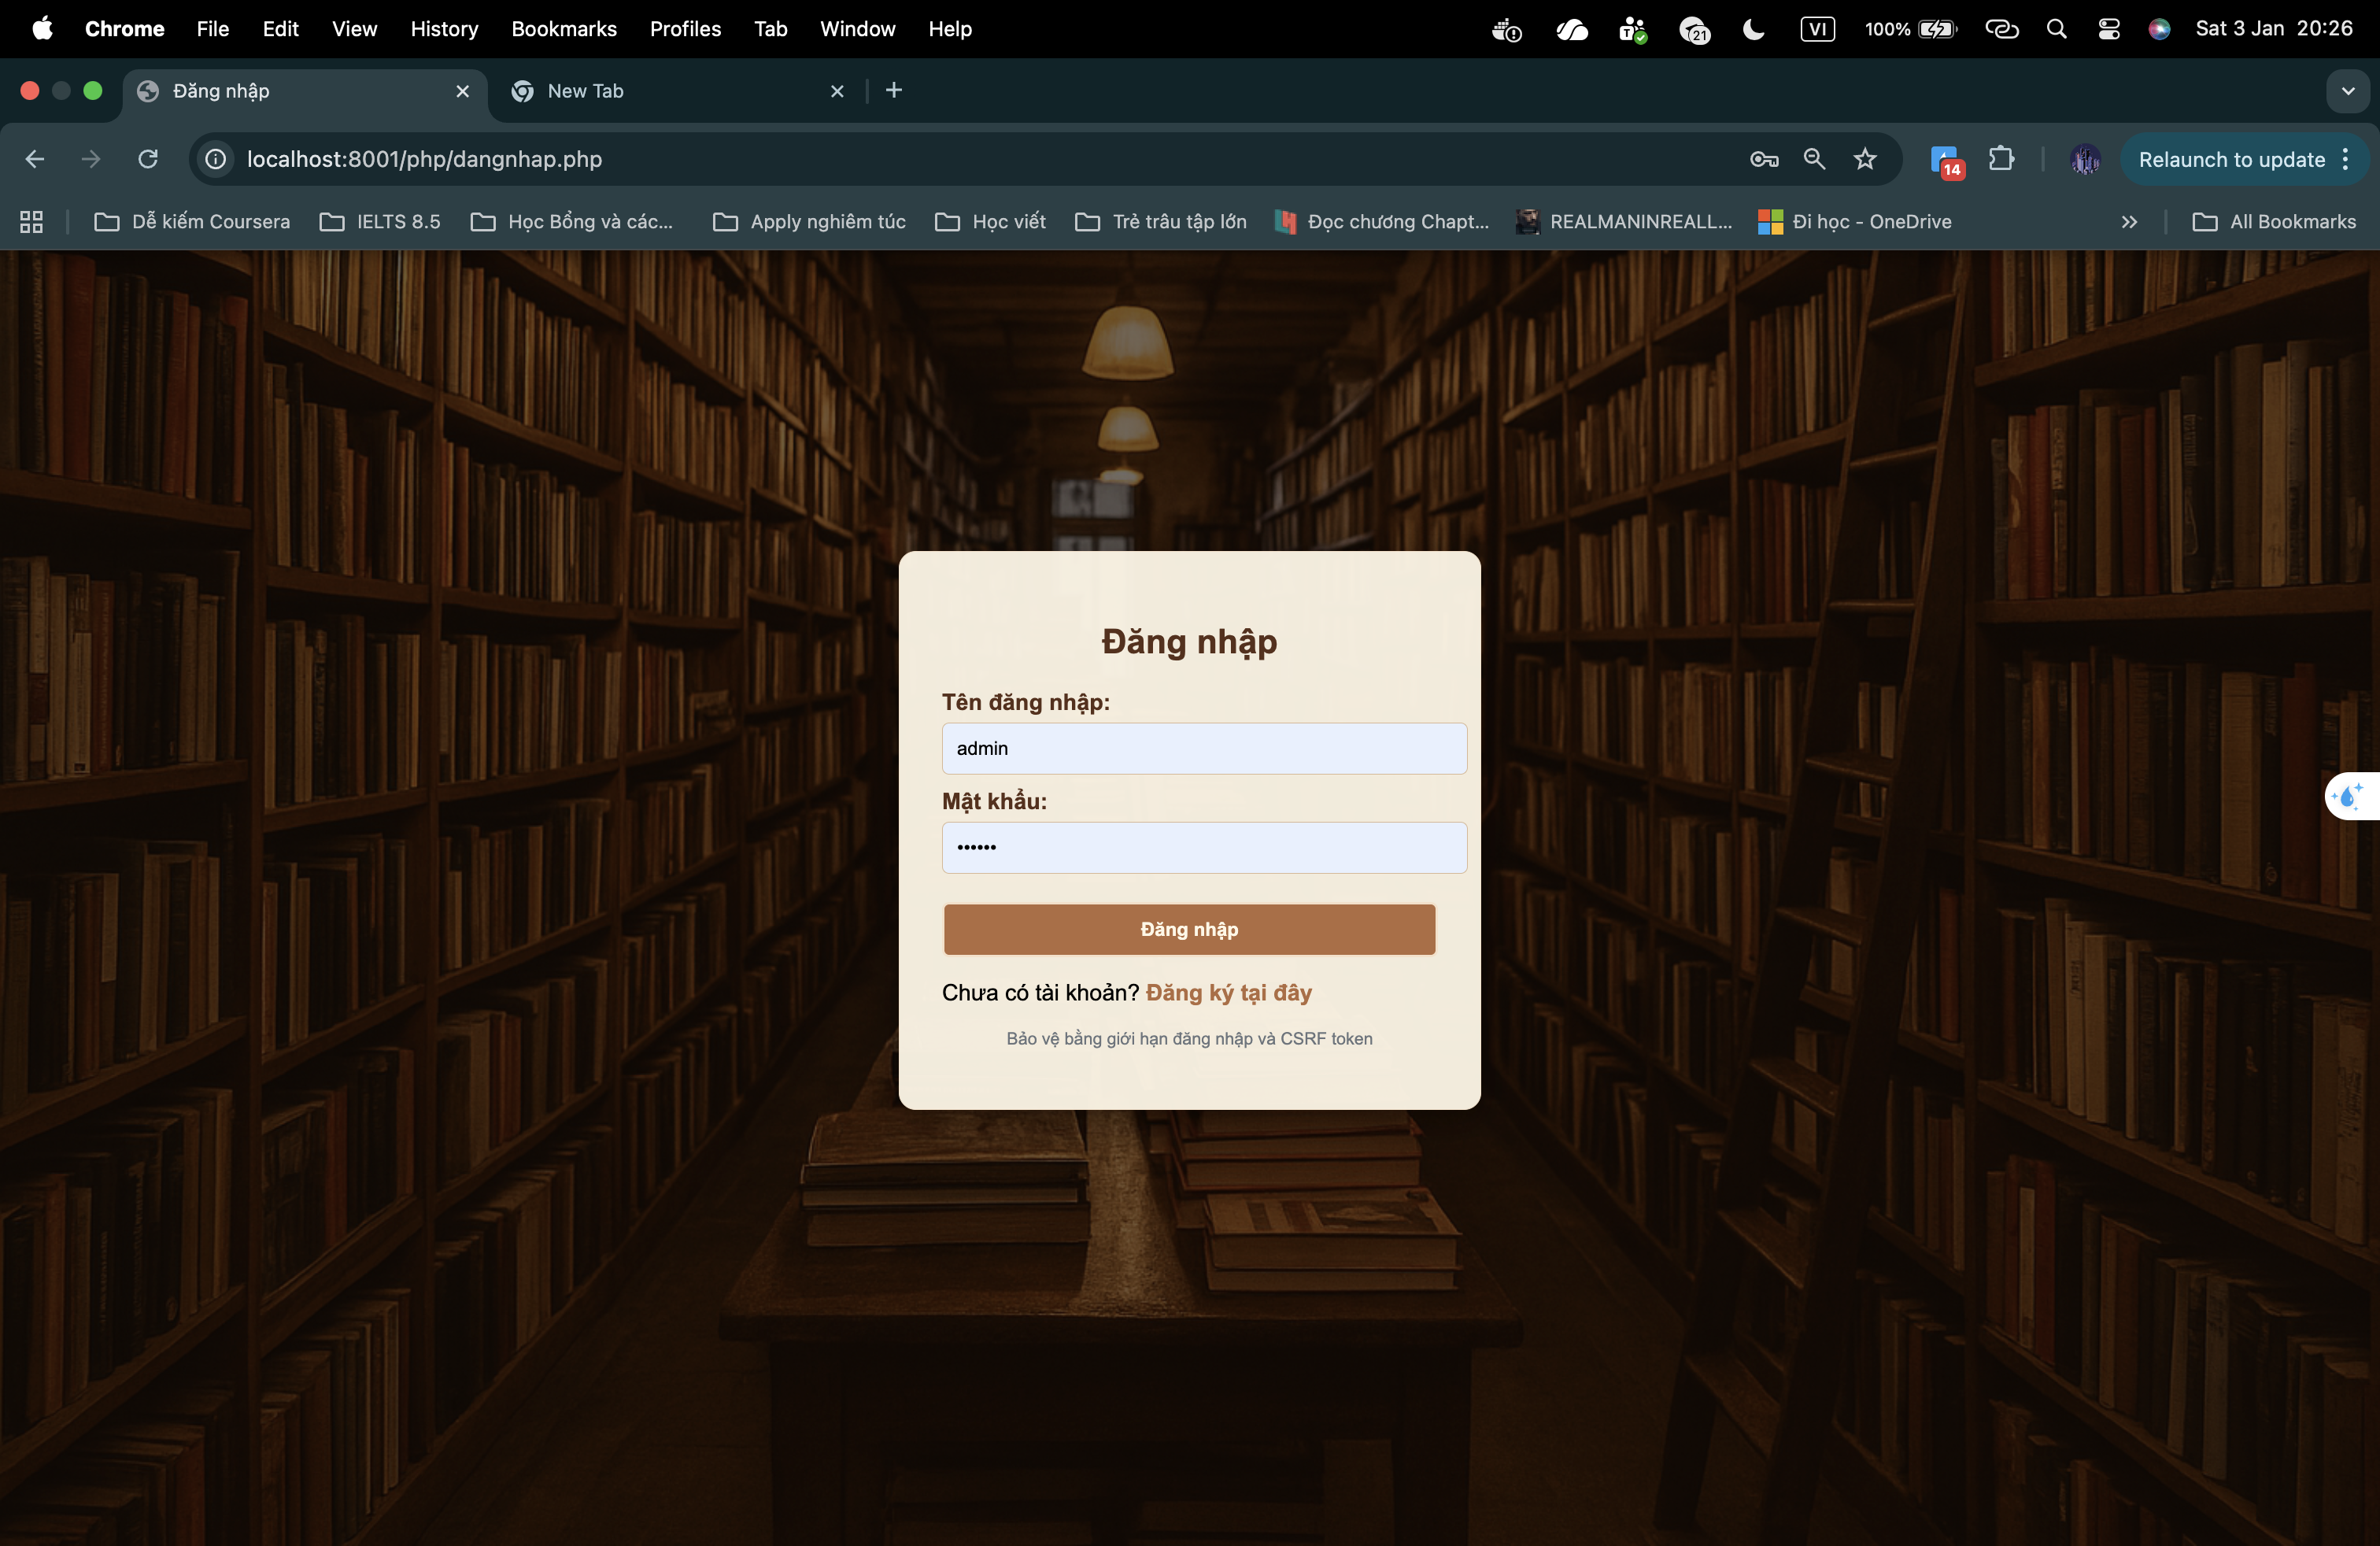
\includegraphics[width=0.85\textwidth]{01_login.png}
    \caption{Giao diện đăng nhập hệ thống}
    \label{fig:login}
\end{figure}

Giao diện đăng nhập hỗ trợ:
\begin{itemize}
    \item Xác thực username/password với bcrypt hash
    \item Phát hiện brute-force attack (lock sau 5 lần thất bại)
    \item Tạo JWT token với thời hạn 24 giờ
    \item Chuyển hướng theo role (admin $\rightarrow$ dashboard, customer $\rightarrow$ danhsachsach)
\end{itemize}

\subsection{Dashboard thống kê (Admin)}

\begin{figure}[H]
    \centering
    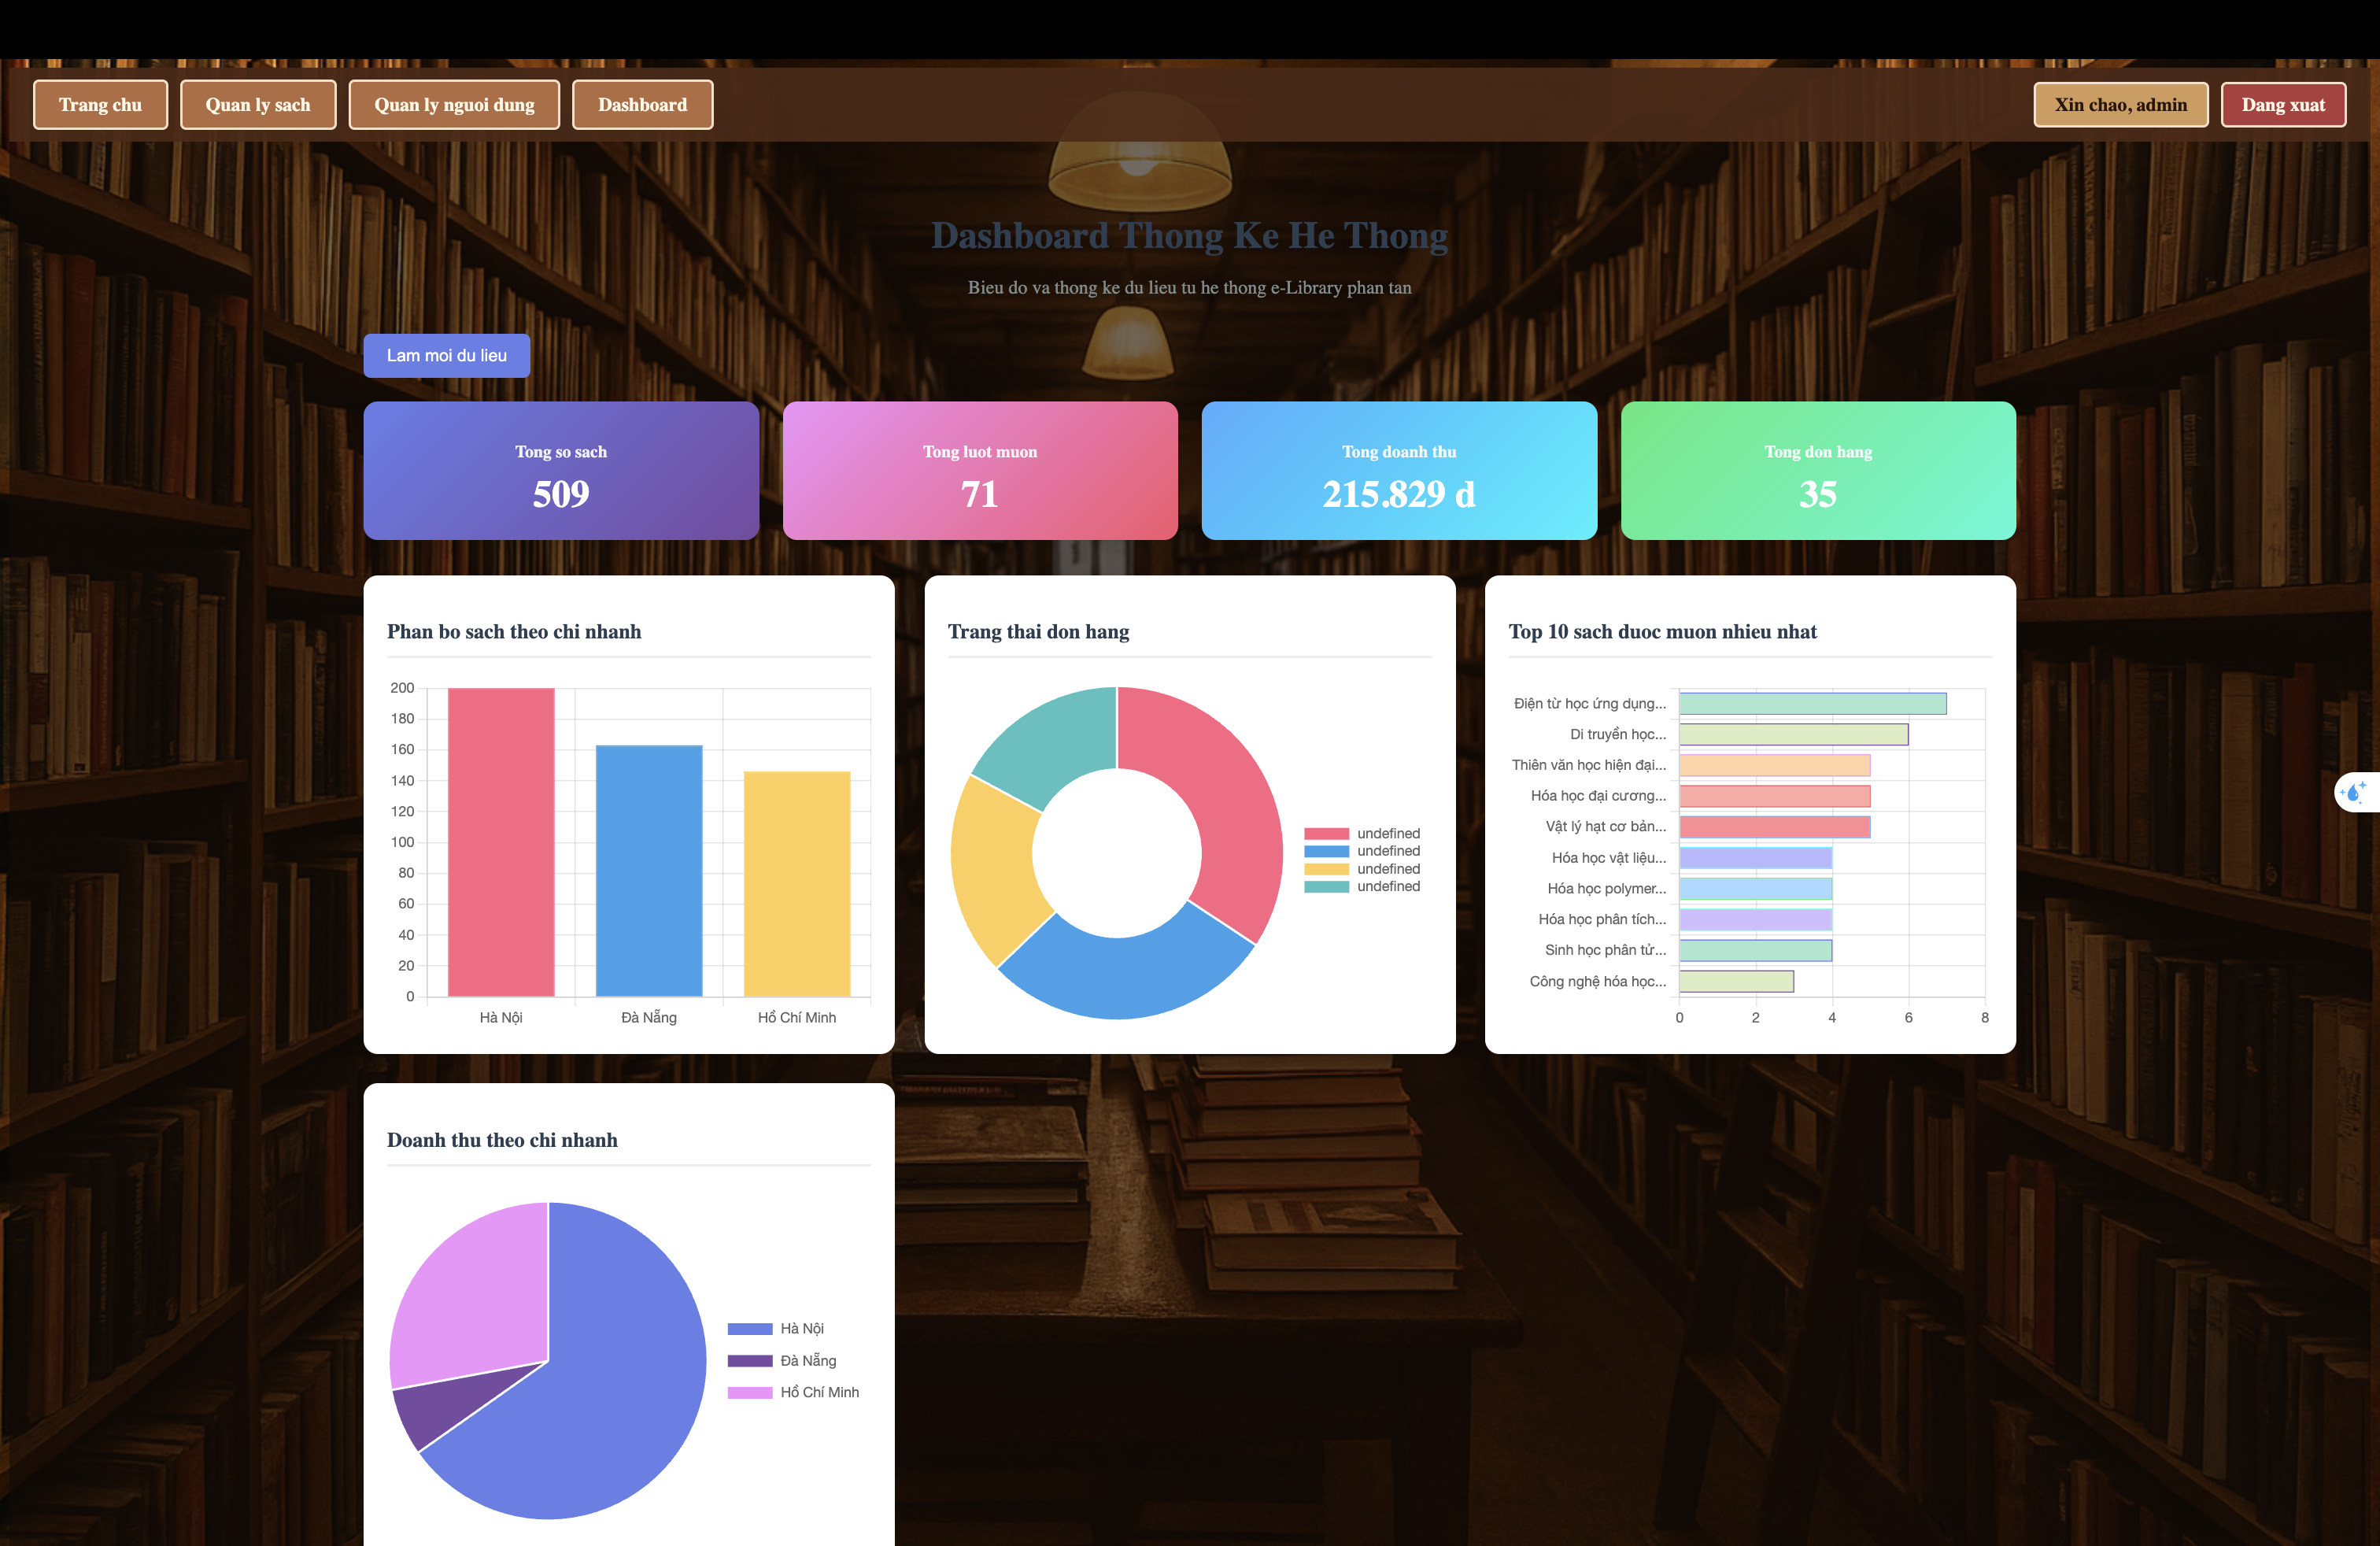
\includegraphics[width=\textwidth]{02_dashboard.png}
    \caption{Dashboard thống kê với biểu đồ Chart.js}
    \label{fig:dashboard}
\end{figure}

Dashboard hiển thị:
\begin{itemize}
    \item Tổng số sách, người dùng, đơn mượn qua cards
    \item Biểu đồ cột: Sách theo chi nhánh
    \item Biểu đồ tròn: Trạng thái đơn hàng
    \item Dữ liệu lấy từ API \texttt{/api/statistics.php}
\end{itemize}

\subsection{Quản lý sách (Admin)}

\begin{figure}[H]
    \centering
    \includegraphics[width=\textwidth]{03_quanlysach.png}
    \caption{Giao diện CRUD quản lý sách}
    \label{fig:quanlysach}
\end{figure}

\subsection{Quản lý người dùng (Admin)}

\begin{figure}[H]
    \centering
    \includegraphics[width=\textwidth]{04_quanlynguoidung.png}
    \caption{Giao diện quản lý người dùng: Danh sách tổng hợp toàn hệ thống}
    \label{fig:quanlynguoidung}
\end{figure}

Giao diện quản lý người dùng hiện tại hiển thị đầy đủ 42 tài khoản, bao gồm 9 quản trị viên tại "Trung Tâm" và 33 khách hàng được đồng bộ từ các chi nhánh (Hà Nội, Đà Nẵng, TP.HCM).

\begin{figure}[H]
    \centering
    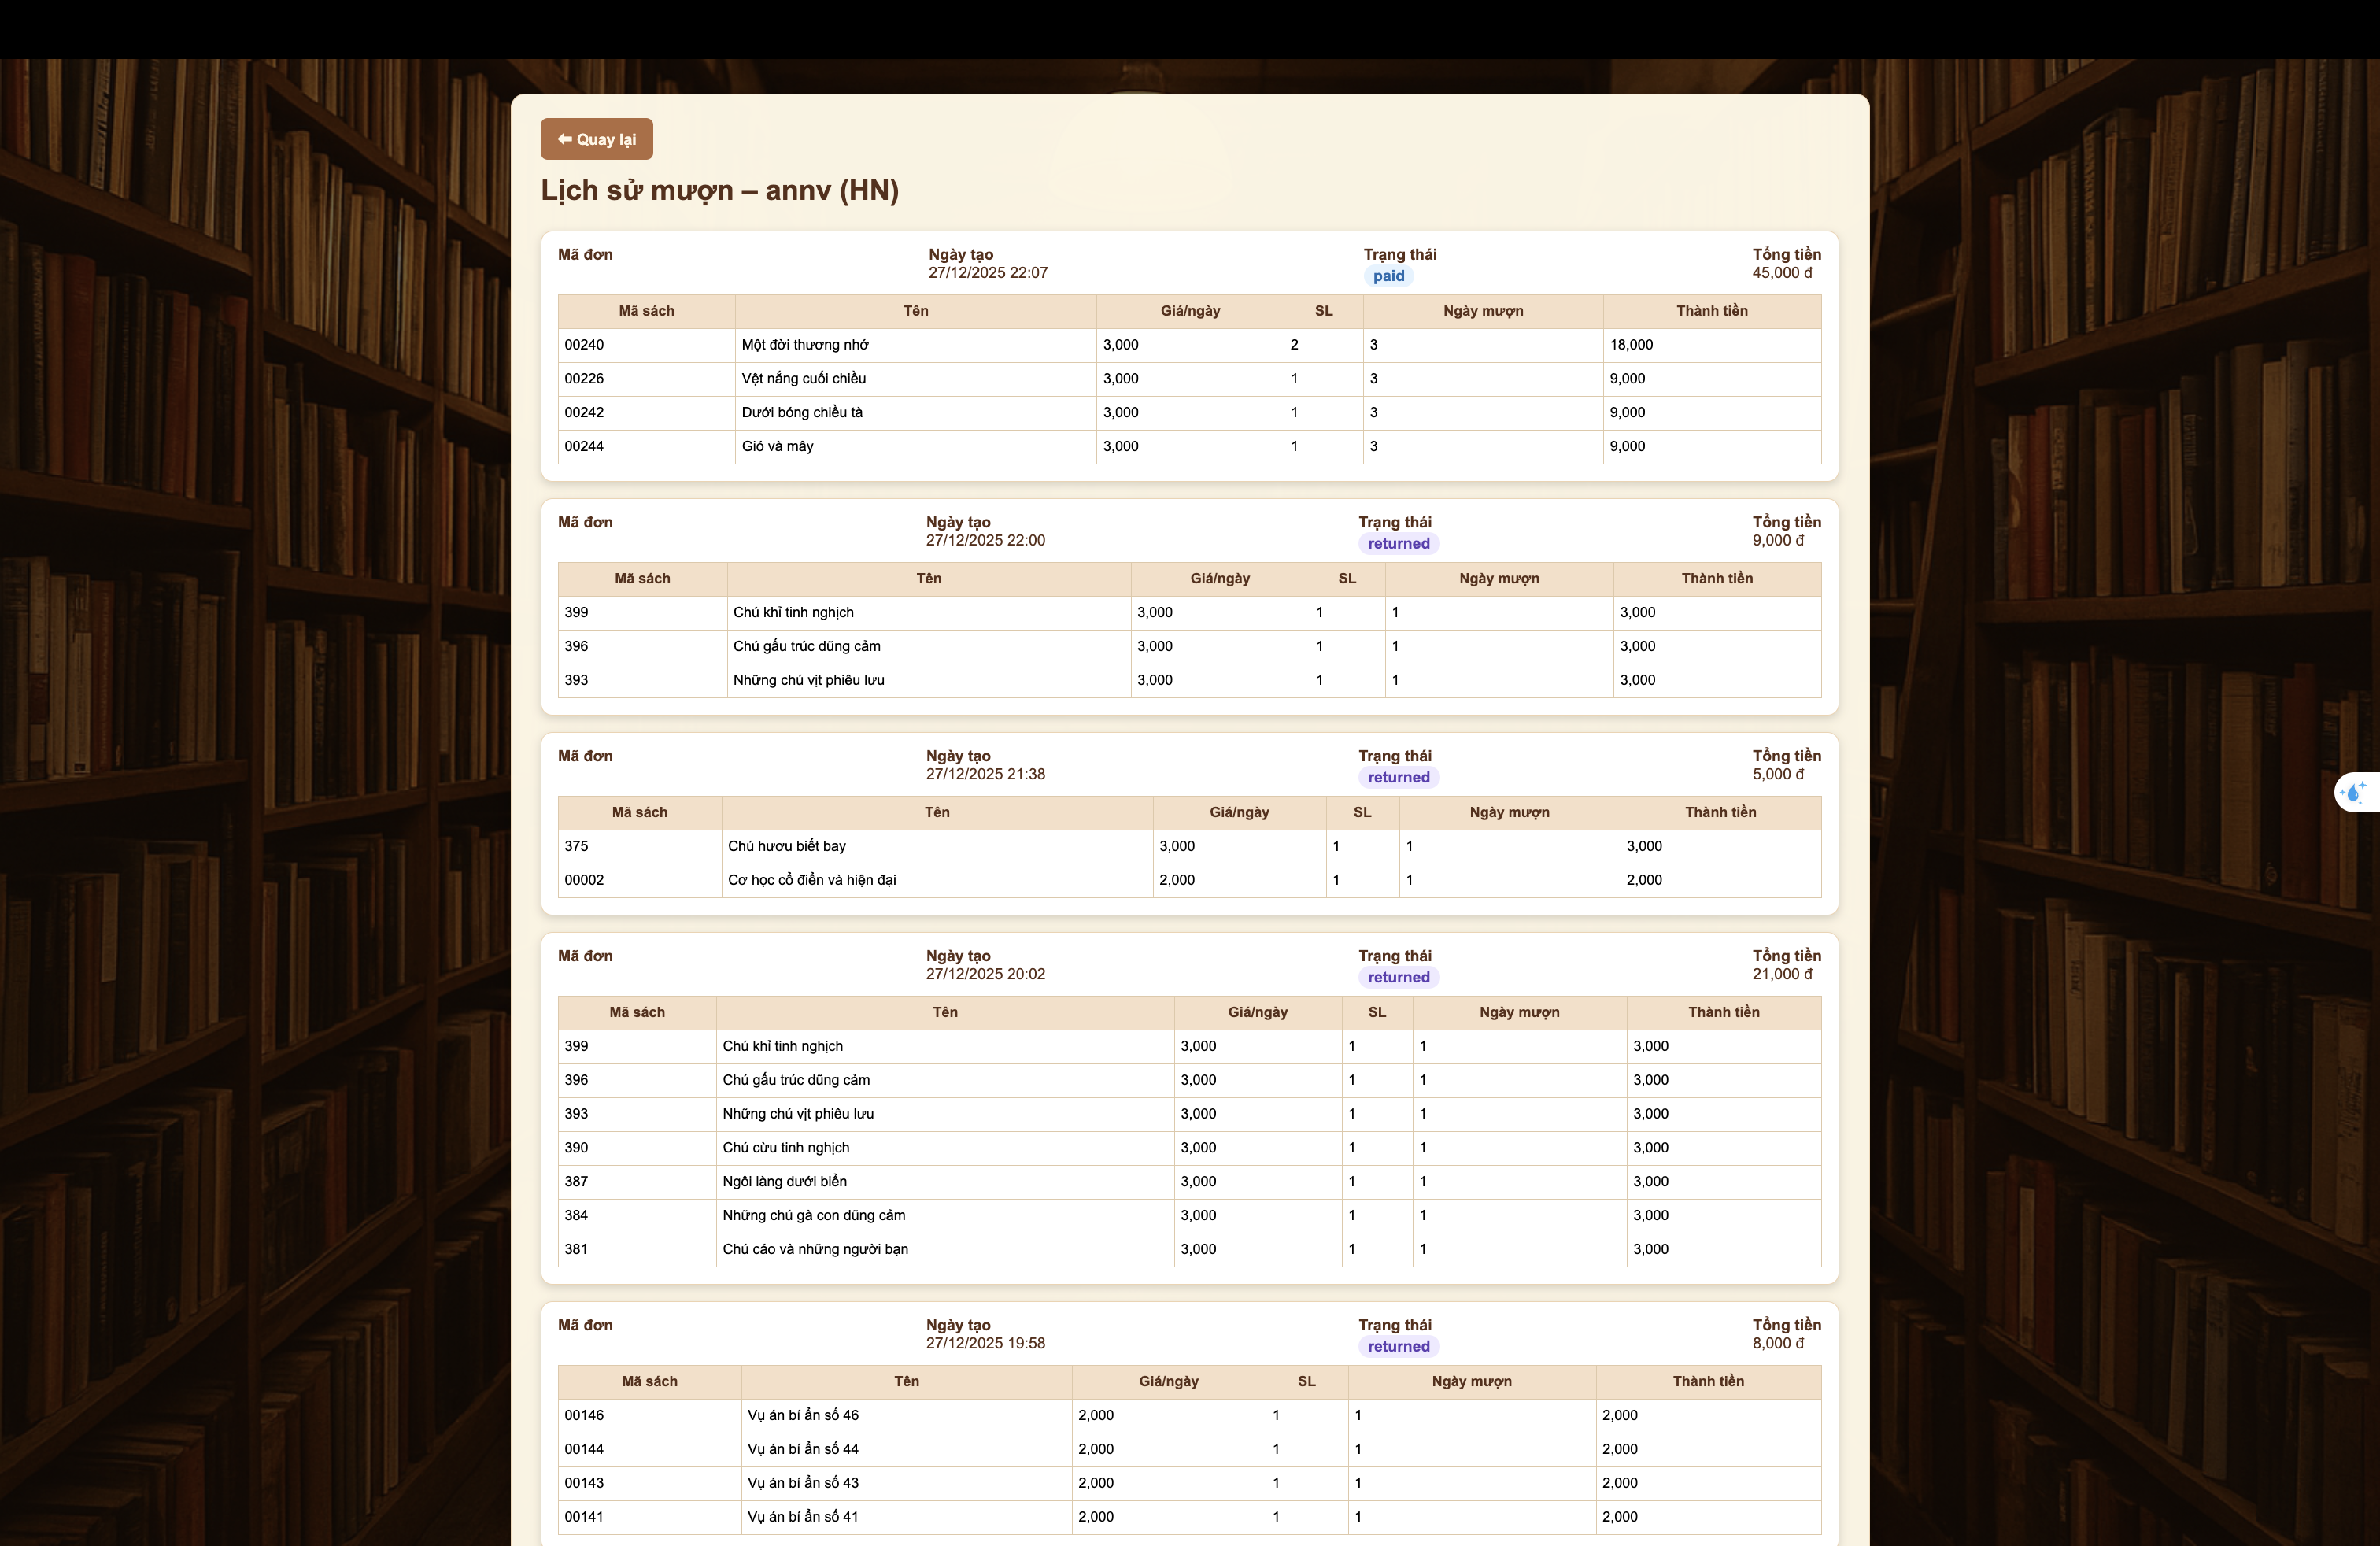
\includegraphics[width=\textwidth]{04_quanlynguoidung_donmuon.png}
    \caption{Chi tiết thống kê đơn mượn: Tổng hợp từ dữ liệu phân tán}
    \label{fig:quanlynguoidung_donmuon}
\end{figure}

Hệ thống tự động tính toán và hiển thị chính xác "Tổng đơn mượn" cho từng người dùng bằng cách cộng gộp dữ liệu từ cơ sở dữ liệu trung tâm và các đơn hàng được đồng bộ từ chi nhánh, đảm bảo tính nhất quán của báo cáo.


\subsection{Danh sách sách (Customer)}

\begin{figure}[H]
    \centering
    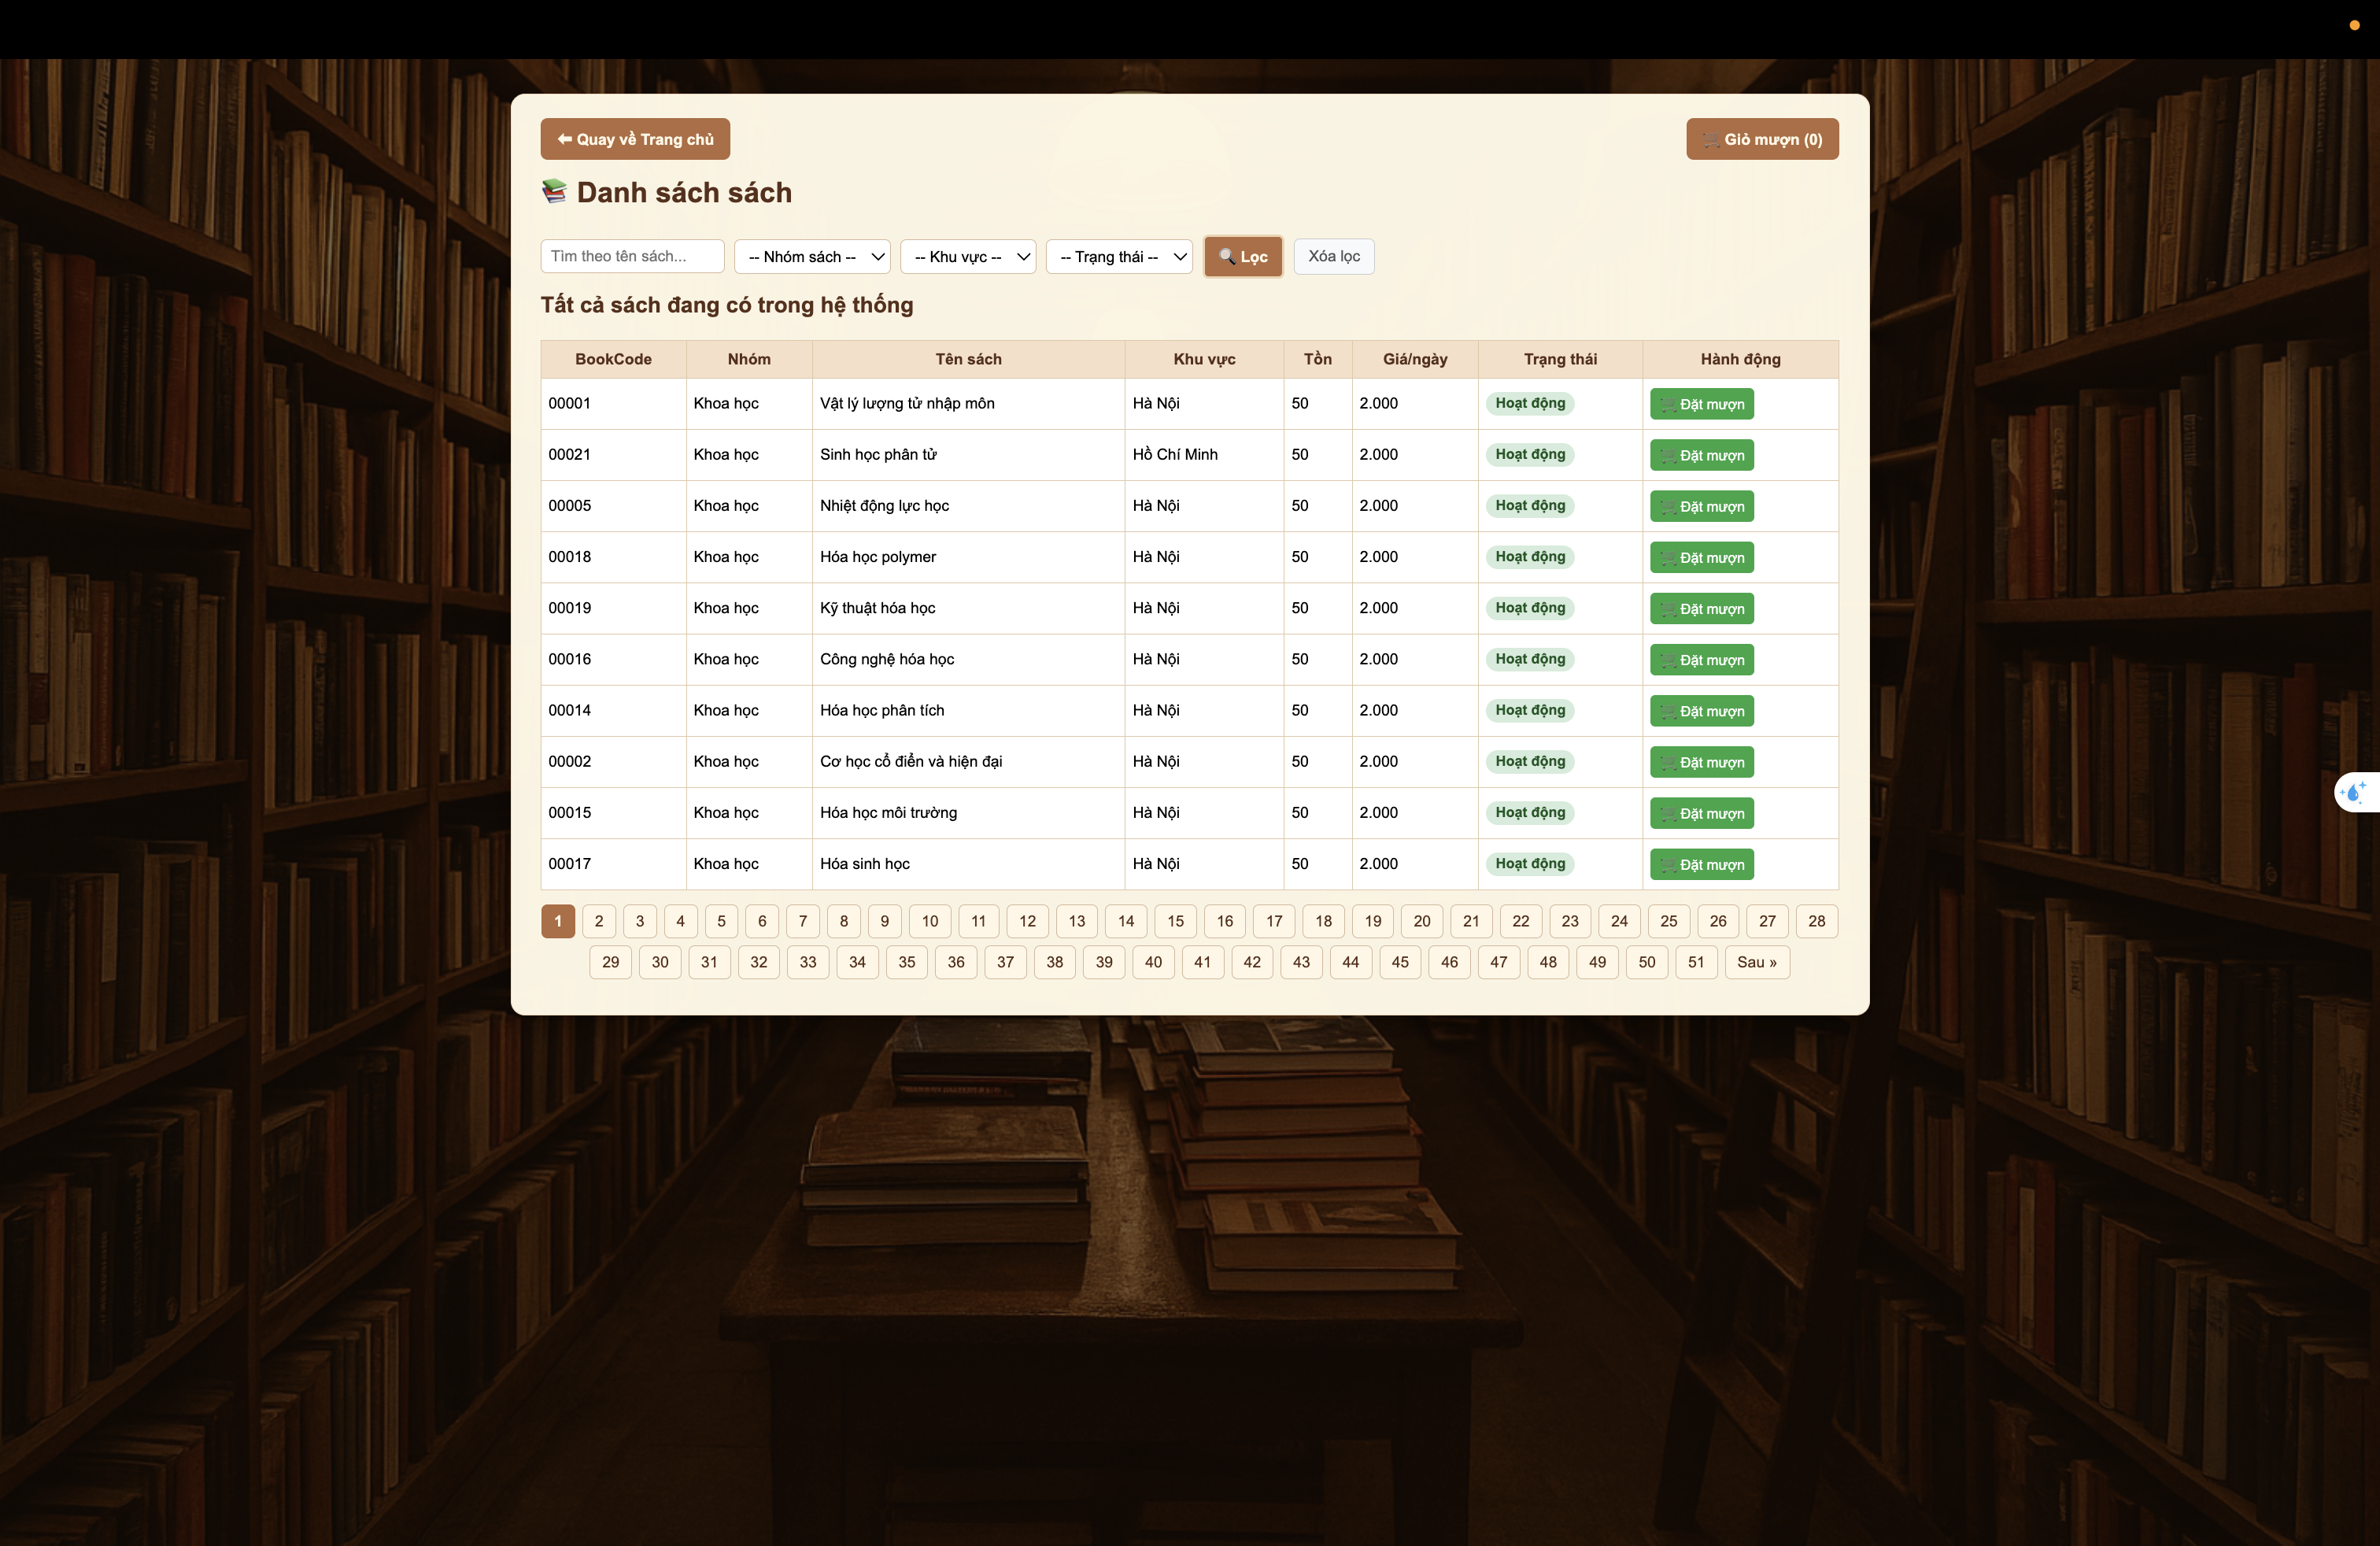
\includegraphics[width=\textwidth]{05_danhsachsach.png}
    \caption{Danh sách sách cho khách hàng}
    \label{fig:danhsachsach}
\end{figure}

\subsection{Giỏ hàng mượn sách}

\begin{figure}[H]
    \centering
    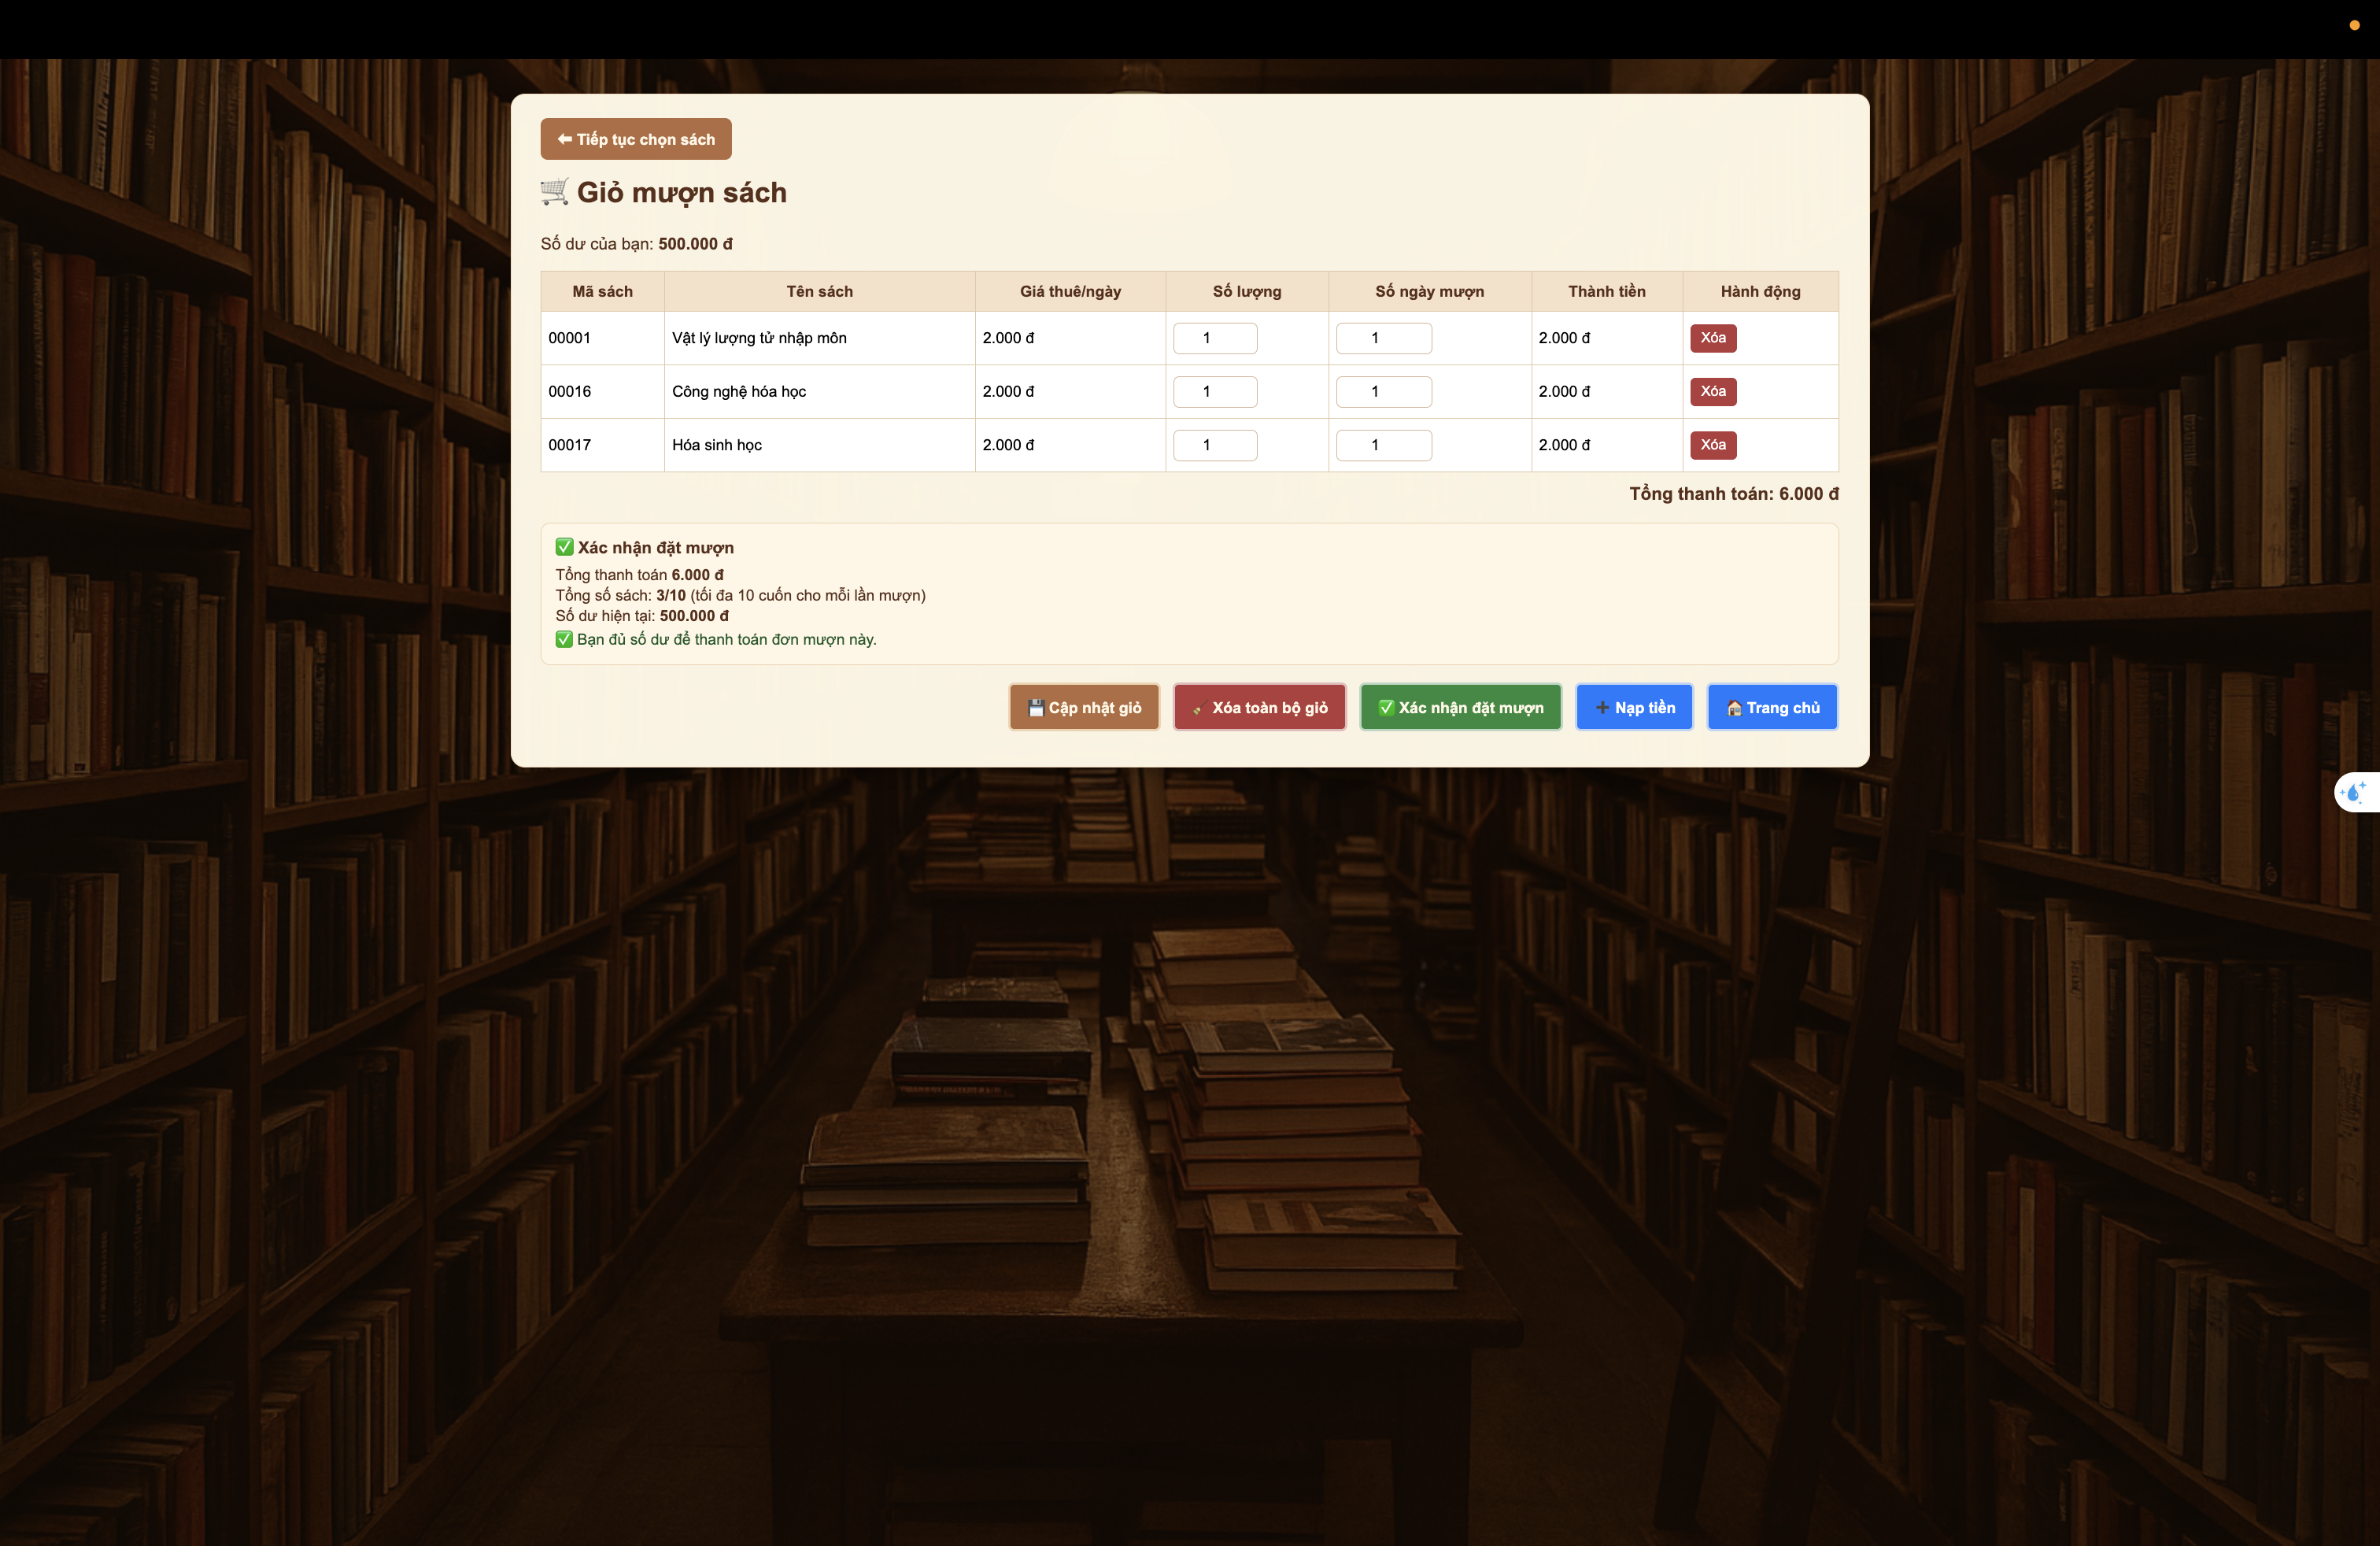
\includegraphics[width=\textwidth]{06_giohang.png}
    \caption{Giao diện giỏ hàng mượn sách}
    \label{fig:giohang}
\end{figure}

\subsection{Dữ liệu Chi nhánh (Mô hình Phân tán)}

\begin{figure}[H]
    \centering
    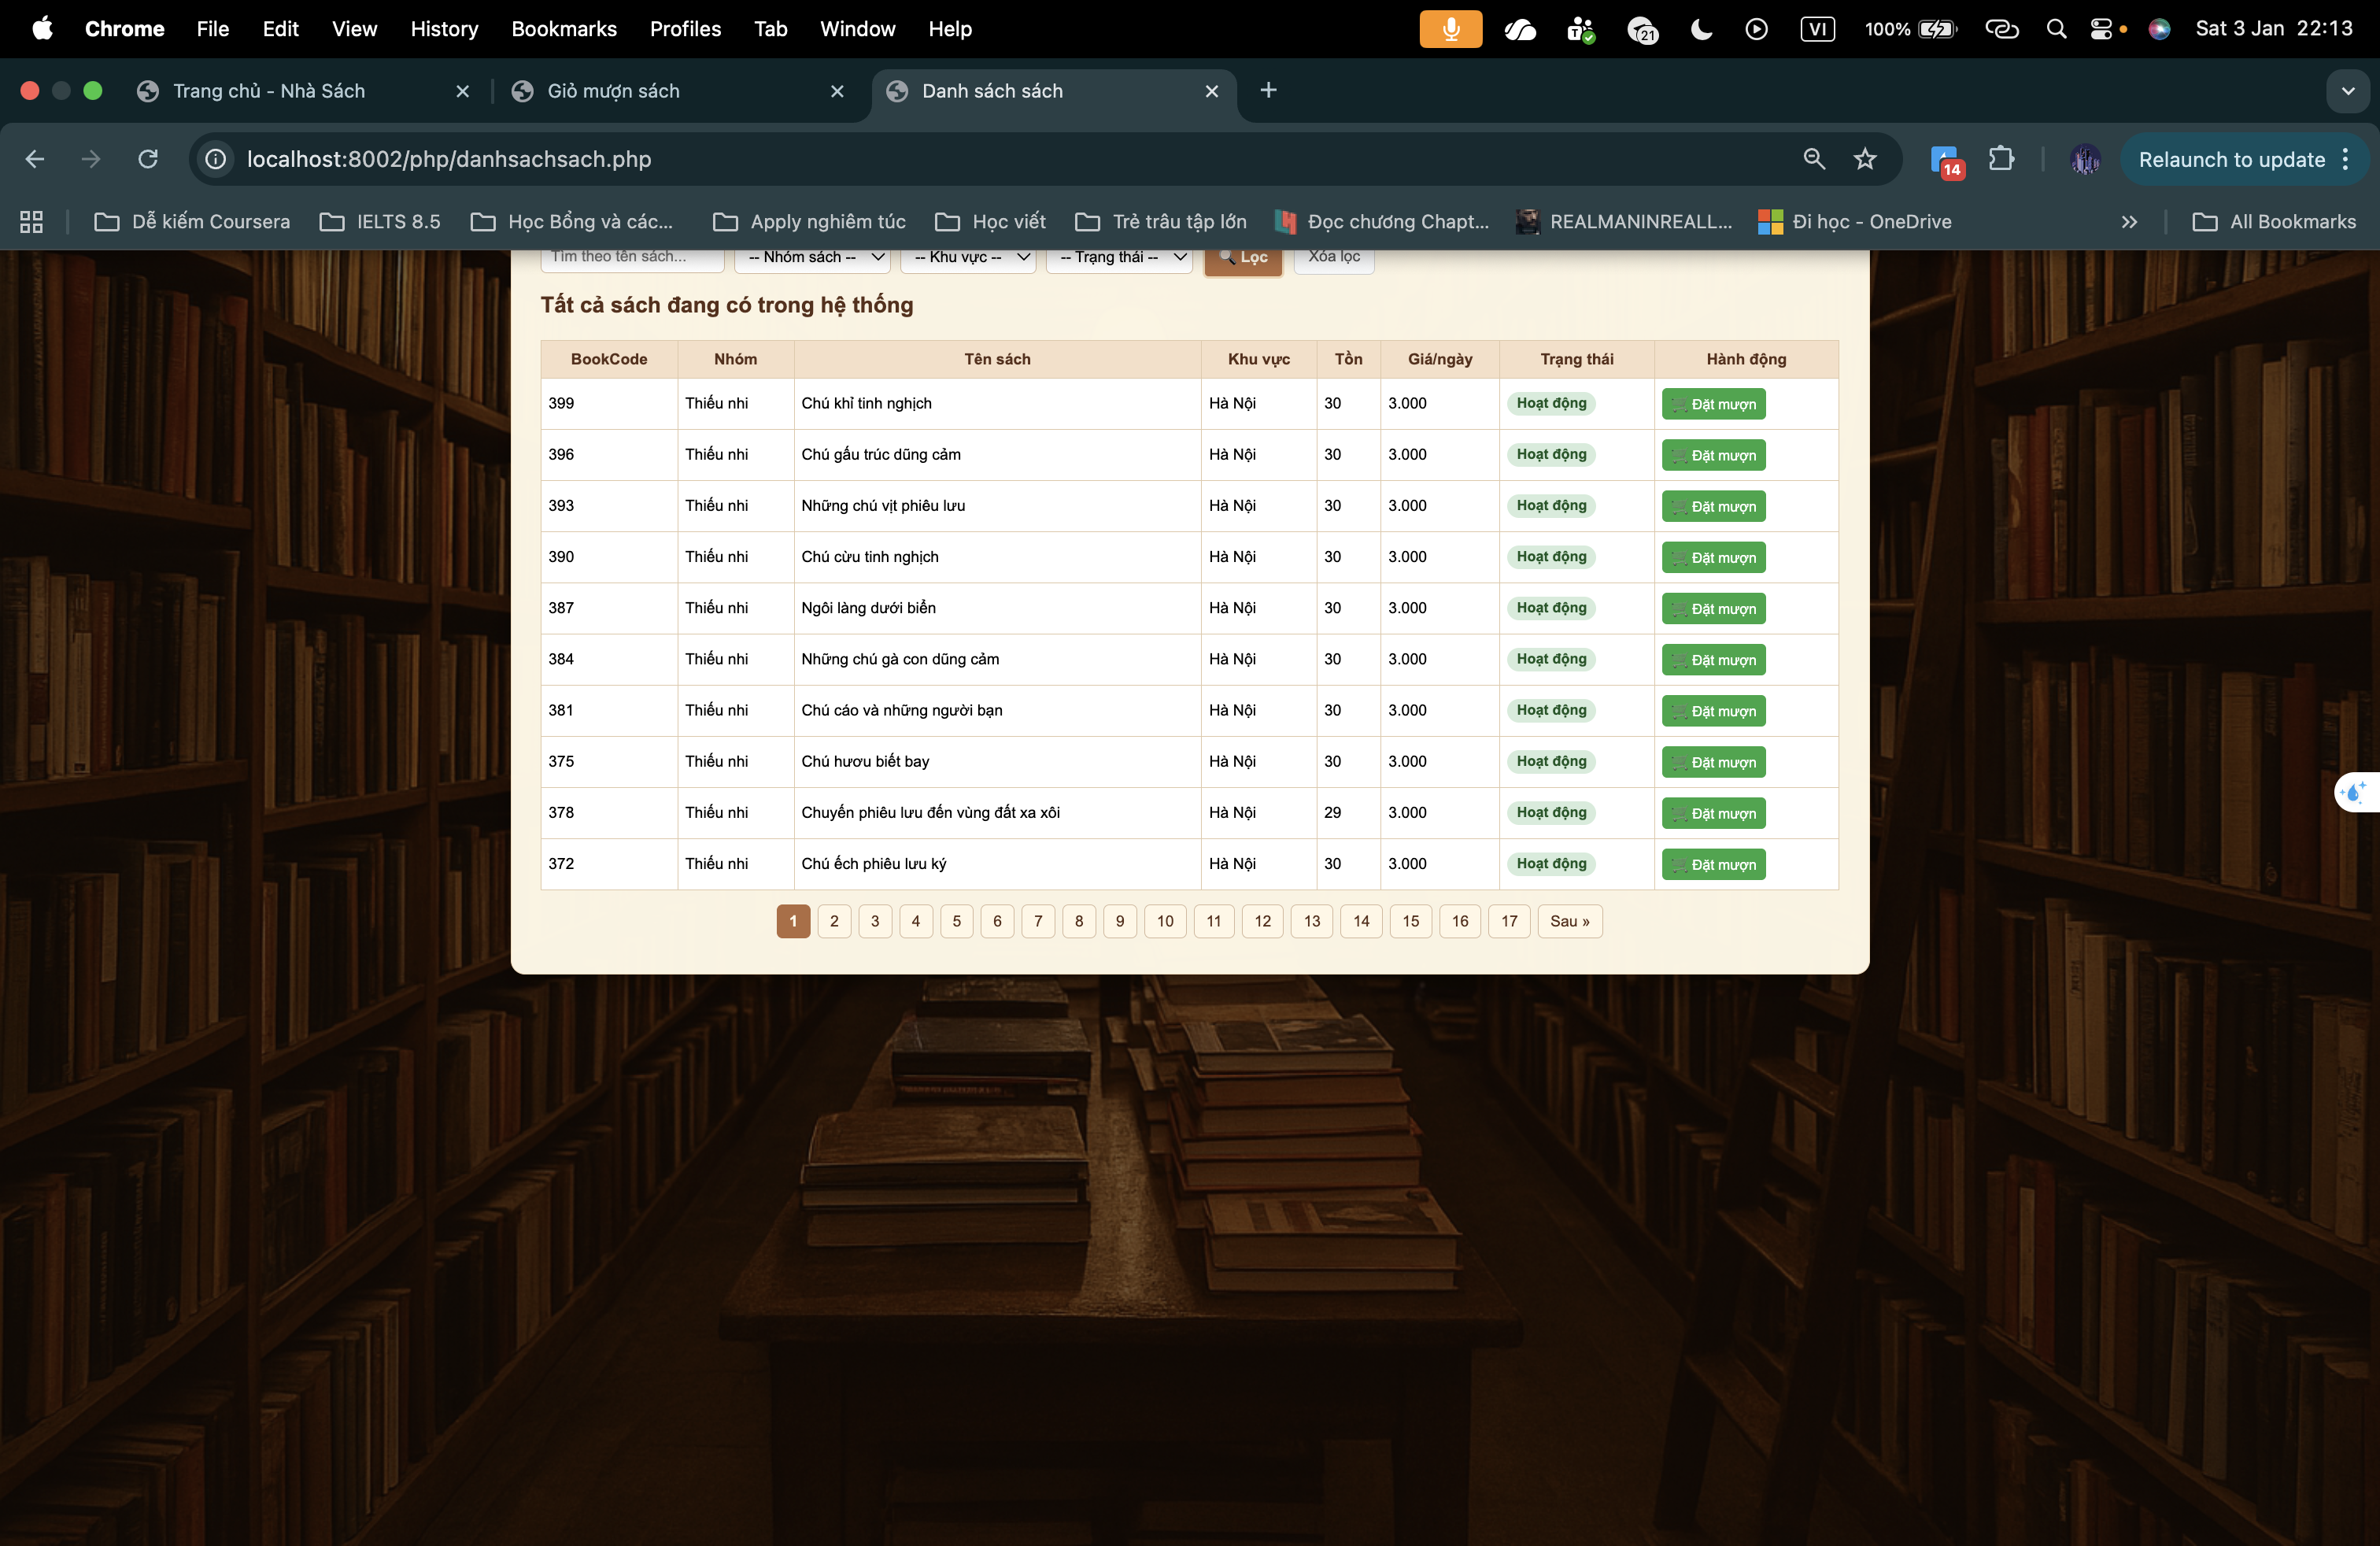
\includegraphics[width=\textwidth]{07_branch_books.png}
    \caption{Danh sách sách tại chi nhánh Hà Nội}
    \label{fig:branch_books}
\end{figure}

\begin{figure}[H]
    \centering
    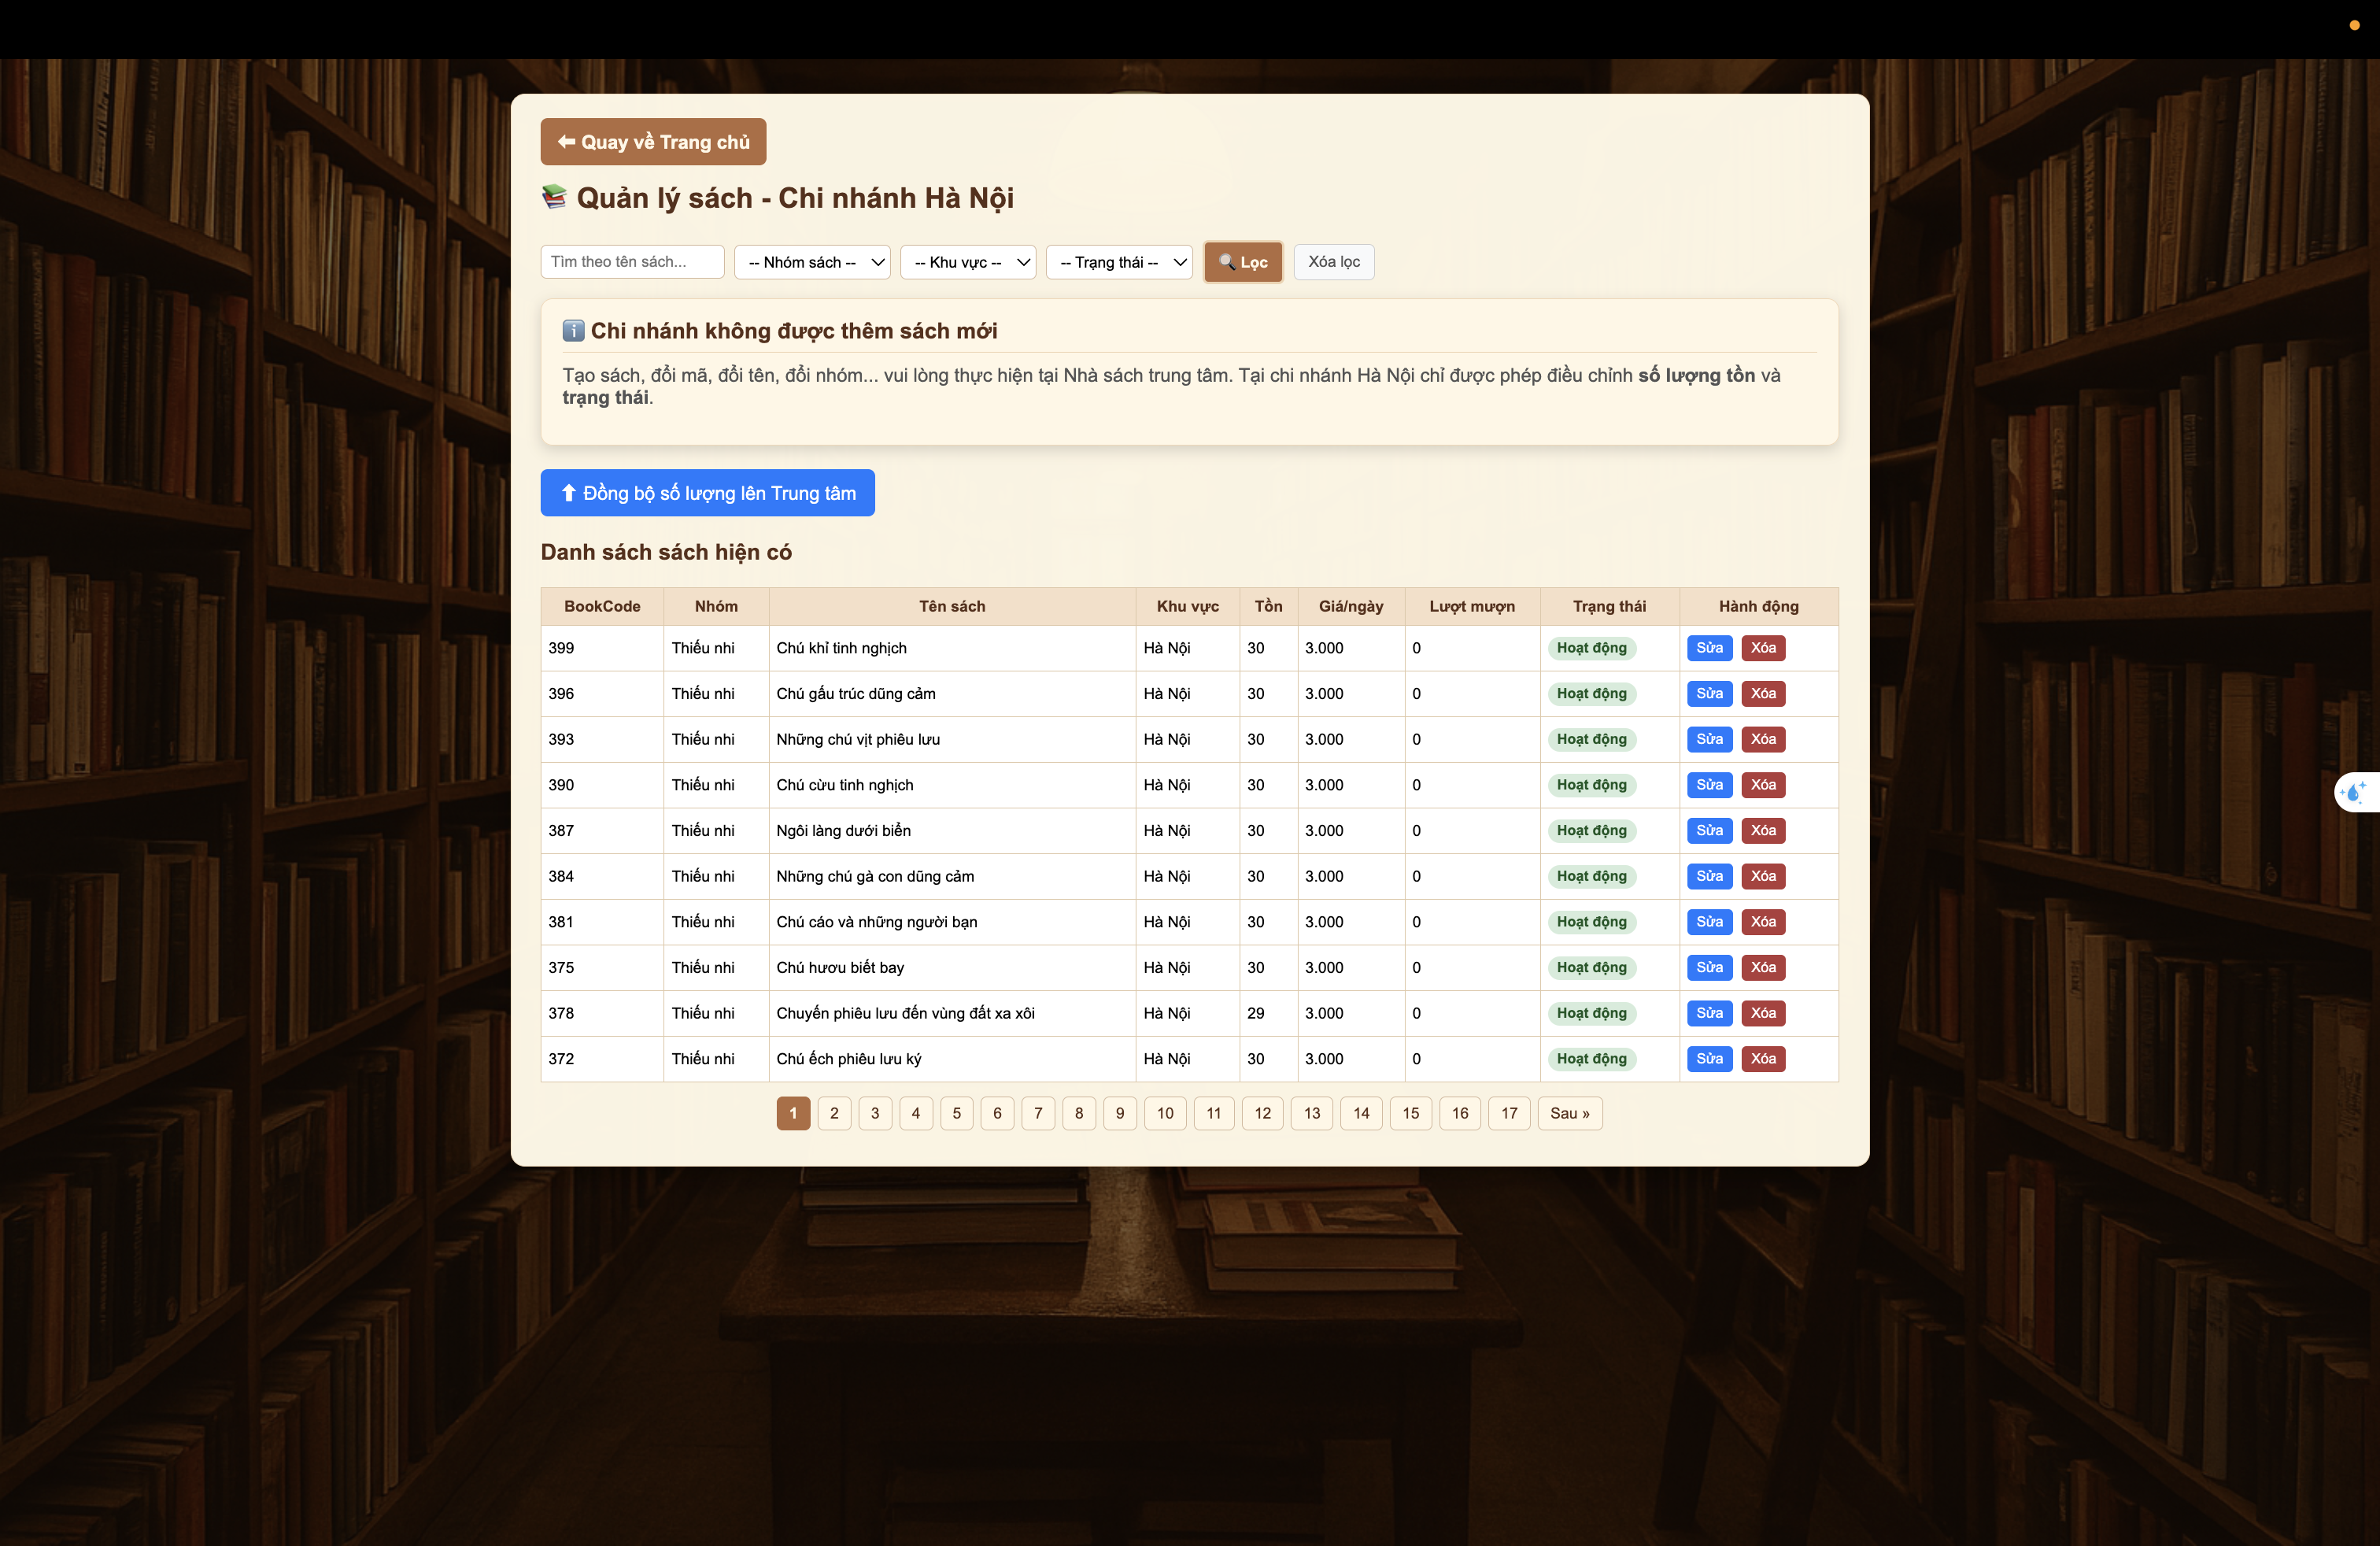
\includegraphics[width=\textwidth]{09_branch_admin.png}
    \caption{Giao diện Admin quản lý tại chi nhánh}
    \label{fig:branch_admin}
\end{figure}

\subsection{Docker Containers}

\begin{figure}[H]
    \centering
    \includegraphics[width=0.8\textwidth]{10_docker.png}
    \caption{Docker Desktop hiển thị MongoDB containers}
    \label{fig:docker}
\end{figure}

\subsection{MongoDB Compass}

\begin{figure}[H]
    \centering
    \includegraphics[width=\textwidth]{11_mongodb_compass.png}
    \caption{MongoDB Compass hiển thị collection books}
    \label{fig:compass}
\end{figure}

\section{Triển khai Aggregation Pipeline}

\subsection{Tổng quan API Statistics}

Hệ thống cung cấp 8 endpoints thống kê sử dụng Aggregation Pipeline trong file \texttt{api/statistics.php}:

\begin{table}[H]
\centering
\caption{Danh sách Aggregation Pipeline endpoints}
\begin{tabular}{|c|l|l|}
\hline
\textbf{\#} & \textbf{Action} & \textbf{Pipeline Stages} \\
\hline
1 & books\_by\_location & \$match, \$group, \$sort, \$project \\
2 & popular\_books & \$match, \$sort, \$limit, \$project \\
3 & revenue\_by\_date & \$match, \$addFields, \$group, \$sort, \$project \\
4 & user\_statistics & \$match, \$group, \$sort, \$limit, \$addFields, \$project \\
5 & user\_details & \$match, \textbf{\$lookup}, \$unwind, \$group, \$sort, \$limit \\
6 & order\_status\_summary & \$group, \$sort, \$project \\
7 & monthly\_trends & \$match, \$addFields, \$group, \$sort, \$project \\
8 & book\_group\_stats & \$match, \textbf{\$facet}, \textbf{\$bucket} \\
\hline
\end{tabular}
\end{table}

\subsection{Endpoint books\_by\_location}

\begin{lstlisting}[language=PHP, caption=statistics.php - books\_by\_location với 4 stages]
case 'books_by_location':
    $pipeline = [
        // Stage 1: $match - Filter active books
        ['$match' => ['status' => ['$ne' => 'deleted']]],

        // Stage 2: $group - Aggregate by location
        ['$group' => [
            '_id' => '$location',
            'totalBooks' => ['$sum' => 1],
            'totalQuantity' => ['$sum' => '$quantity'],
            'avgPricePerDay' => ['$avg' => '$pricePerDay'],
            'totalBorrowCount' => ['$sum' => '$borrowCount']
        ]],

        // Stage 3: $sort - Order by total books
        ['$sort' => ['totalBooks' => -1]],

        // Stage 4: $project - Rename and format fields
        ['$project' => [
            '_id' => 0,
            'location' => '$_id',
            'totalBooks' => 1,
            'totalQuantity' => 1,
            'avgPricePerDay' => ['$round' => ['$avgPricePerDay', 0]],
            'totalBorrowCount' => 1
        ]]
    ];

    $result = $db->books->aggregate($pipeline)->toArray();
\end{lstlisting}

\subsection{Endpoint user\_details với \$lookup JOIN}

Đây là endpoint quan trọng nhất, thể hiện khả năng JOIN giữa các collections trong MongoDB:

\begin{lstlisting}[language=PHP, caption=statistics.php - user\_details với \$lookup]
case 'user_details':
    $pipeline = [
        // Stage 1: Match completed orders
        ['$match' => ['status' => ['$in' => ['paid', 'success', 'returned']]]],

        // Stage 2: $lookup - LEFT OUTER JOIN with users collection
        ['$lookup' => [
            'from' => 'users',           // Target collection
            'localField' => 'user_id',   // Field in orders
            'foreignField' => '_id',     // Field in users
            'as' => 'user_info'          // Output array
        ]],

        // Stage 3: $unwind - Flatten user_info array
        ['$unwind' => [
            'path' => '$user_info',
            'preserveNullAndEmptyArrays' => true
        ]],

        // Stage 4: Group by user with joined info
        ['$group' => [
            '_id' => '$user_id',
            'username' => ['$first' => '$username'],
            'email' => ['$first' => '$user_info.email'],
            'fullname' => ['$first' => '$user_info.fullname'],
            'role' => ['$first' => '$user_info.role'],
            'totalOrders' => ['$sum' => 1],
            'totalSpent' => ['$sum' => '$total_amount']
        ]],

        ['$sort' => ['totalSpent' => -1]],
        ['$limit' => 20]
    ];

    $result = $db->orders->aggregate($pipeline)->toArray();
\end{lstlisting}

\subsection{Endpoint book\_group\_stats với \$facet và \$bucket}

\begin{lstlisting}[language=PHP, caption=statistics.php - Multi-faceted statistics]
case 'book_group_stats':
    $pipeline = [
        ['$match' => ['status' => ['$ne' => 'deleted']]],

        ['$facet' => [
            // Facet 1: Statistics by book group
            'byGroup' => [
                ['$group' => [
                    '_id' => '$bookGroup',
                    'count' => ['$sum' => 1],
                    'totalQuantity' => ['$sum' => '$quantity']
                ]],
                ['$sort' => ['count' => -1]]
            ],

            // Facet 2: Overall summary
            'summary' => [
                ['$group' => [
                    '_id' => null,
                    'totalBooks' => ['$sum' => 1],
                    'avgPrice' => ['$avg' => '$pricePerDay'],
                    'totalBorrows' => ['$sum' => '$borrowCount']
                ]]
            ],

            // Facet 3: Price distribution with $bucket
            'priceRanges' => [
                ['$bucket' => [
                    'groupBy' => '$pricePerDay',
                    'boundaries' => [0, 5000, 10000, 20000, 50000, 100000],
                    'default' => 'Other',
                    'output' => ['count' => ['$sum' => 1]]
                ]]
            ]
        ]]
    ];
\end{lstlisting}

\section{Triển khai Map-Reduce}

\subsection{Tổng quan API Map-Reduce}

File \texttt{api/mapreduce.php} cung cấp 5 Map-Reduce operations:

\begin{table}[H]
\centering
\caption{Danh sách Map-Reduce operations}
\begin{tabular}{|c|l|l|}
\hline
\textbf{\#} & \textbf{Action} & \textbf{Mô tả} \\
\hline
1 & borrow\_stats & Thống kê mượn sách theo bookCode \\
2 & revenue\_by\_user & Doanh thu theo user \\
3 & books\_by\_category & Sách theo thể loại \\
4 & daily\_activity & Hoạt động theo ngày \\
5 & location\_performance & Hiệu suất theo chi nhánh \\
\hline
\end{tabular}
\end{table}

\subsection{Map-Reduce: borrow\_stats}

\begin{lstlisting}[language=PHP, caption=mapreduce.php - Borrowing statistics]
case 'borrow_stats':
    // Map function: emit bookCode with borrow info
    $mapFunction = new MongoDB\BSON\Javascript('
        function() {
            if (this.items && Array.isArray(this.items)) {
                for (var i = 0; i < this.items.length; i++) {
                    var item = this.items[i];
                    emit(item.bookCode, {
                        count: 1,
                        quantity: item.quantity || 1,
                        revenue: item.subtotal || 0,
                        bookName: item.bookName || "Unknown"
                    });
                }
            }
        }
    ');

    // Reduce function: aggregate values
    $reduceFunction = new MongoDB\BSON\Javascript('
        function(key, values) {
            var result = { count: 0, quantity: 0, revenue: 0, bookName: "" };
            for (var i = 0; i < values.length; i++) {
                result.count += values[i].count;
                result.quantity += values[i].quantity;
                result.revenue += values[i].revenue;
                if (values[i].bookName !== "Unknown") {
                    result.bookName = values[i].bookName;
                }
            }
            return result;
        }
    ');

    // Finalize function: calculate averages
    $finalizeFunction = new MongoDB\BSON\Javascript('
        function(key, reducedValue) {
            reducedValue.avgQuantityPerOrder = reducedValue.count > 0
                ? reducedValue.quantity / reducedValue.count : 0;
            return reducedValue;
        }
    ');

    $result = $db->command([
        'mapReduce' => 'orders',
        'map' => $mapFunction,
        'reduce' => $reduceFunction,
        'finalize' => $finalizeFunction,
        'out' => ['inline' => 1],
        'query' => ['status' => ['$in' => ['paid', 'success', 'returned']]]
    ]);
\end{lstlisting}

\section{Kiểm thử hệ thống}

\subsection{Kịch bản 1: Kiểm thử hiển thị dữ liệu}

\textbf{Mục đích:} Đảm bảo dữ liệu hiển thị đúng tại mỗi chi nhánh.

\textbf{Kết quả:}
\begin{table}[H]
\centering
\caption{Kết quả kiểm thử hiển thị dữ liệu}
\begin{tabular}{|l|c|c|c|c|}
\hline
\textbf{Chi nhánh} & \textbf{Port} & \textbf{Sách} & \textbf{Người dùng} & \textbf{Đơn mượn} \\
\hline
Central Hub & 8001 & 509 & 42 & 111 \\
Hà Nội & 8002 & 200 & 13 & 46 \\
Đà Nẵng & 8003 & 163 & 12 & 16 \\
TP.HCM & 8004 & 146 & 11 & 14 \\
\hline
\textbf{Tổng} & & \textbf{1.018} & \textbf{78} & \textbf{187} \\
\hline
\end{tabular}
\end{table}

\textbf{Đánh giá:} \textcolor{green}{PASS} - Dữ liệu hiển thị đúng theo từng database.

\subsection{Kịch bản 2: Kiểm thử ghi và đồng bộ}

\textbf{Mục đích:} Đảm bảo dữ liệu đồng bộ từ PRIMARY sang SECONDARY.

\textbf{Các bước:}
\begin{enumerate}
    \item Thêm sách mới tại Central Hub
    \item Kiểm tra sách xuất hiện tại mongo2, mongo3
    \item Đo replication lag
\end{enumerate}

\textbf{Kết quả:}
\begin{itemize}
    \item Ghi vào PRIMARY: Thành công
    \item Replication lag: 50-200ms
    \item Dữ liệu nhất quán: OK
\end{itemize}

\textbf{Đánh giá:} \textcolor{green}{PASS}

\subsection{Kịch bản 3: Kiểm thử Failover}

\textbf{Mục đích:} Đảm bảo hệ thống tự động phục hồi khi PRIMARY gặp sự cố.

\textbf{Các bước:}
\begin{lstlisting}[language=bash, caption=Script kiểm thử Failover]
# 1. Check current status
docker exec mongo1 mongosh --eval "rs.status().members.map(m => m.stateStr)"

# 2. Stop PRIMARY
docker stop mongo1

# 3. Wait for election (10-15s)
sleep 15

# 4. Check new PRIMARY
docker exec mongo2 mongosh --eval "rs.status().members.map(m => m.stateStr)"

# 5. Restart old PRIMARY
docker start mongo1
\end{lstlisting}

\textbf{Kết quả:}
\begin{itemize}
    \item Phát hiện node hỏng: $\sim$10 giây
    \item Bầu chọn PRIMARY mới: $\sim$5 giây
    \item Tổng thời gian gián đoạn: \textbf{10-15 giây}
    \item Hệ thống tiếp tục hoạt động: OK
\end{itemize}

\textbf{Đánh giá:} \textcolor{green}{PASS}

\subsection{Kịch bản 4: Đo lường hiệu năng truy vấn (Benchmark)}

Để đánh giá hiệu năng thực tế của hệ thống, nhóm đã xây dựng một bộ công cụ benchmark với 10 kịch bản truy vấn khác nhau, bao gồm cả các thao tác đọc và ghi. Mỗi kịch bản được thực hiện lặp lại 50 lần (iterations) trên dữ liệu thực của hệ thống để đảm bảo độ chính xác của kết quả đo.

Môi trường thử nghiệm:
\begin{itemize}
    \item \textbf{Phiên bản MongoDB:} 8.0.16 (Community Edition)
    \item \textbf{Dữ liệu thử nghiệm:} 509 cuốn sách, 42 người dùng trong cơ sở dữ liệu Nhasach
    \item \textbf{Số lần lặp:} 50 iterations cho mỗi test case
    \item \textbf{Chế độ kết nối:} Standalone (localhost:27017)
\end{itemize}

\begin{figure}[H]
    \centering
    \includegraphics[width=\textwidth]{12_terminal_benchmark.png}
    \caption{Kết quả benchmark trong Terminal - hiển thị thời gian thực thi và throughput của từng loại truy vấn}
    \label{fig:benchmark}
\end{figure}

Bảng \ref{tab:benchmark} tổng hợp kết quả benchmark với dữ liệu thực, được sắp xếp theo thứ tự từ nhanh nhất đến chậm nhất:

\begin{table}[H]
\centering
\caption{Kết quả benchmark hiệu năng (dữ liệu thực)}
\label{tab:benchmark}
\begin{tabular}{|l|c|c|c|}
\hline
\textbf{Loại truy vấn} & \textbf{TB (ms)} & \textbf{Tổng (ms)} & \textbf{Ops/giây} \\
\hline
Truy vấn khoảng + Sắp xếp (Range Query + Sort) & \textbf{0.880} & 44 & 1,136 \\
Truy vấn kết hợp (Compound Query) & 0.980 & 49 & 1,020 \\
Tra cứu điểm (Point Lookup by bookCode) & 1.040 & 52 & 962 \\
Truy vấn đa vùng (Cross-Shard Query) & 1.920 & 96 & 521 \\
Cập nhật (\$inc + \$set) & 2.160 & 108 & 463 \\
Tìm kiếm toàn văn (Text Search) & 3.200 & 160 & 313 \\
Ghi dữ liệu (Insert + Delete) & 5.680 & 284 & 176 \\
Tổng hợp \$facet (3 pipeline song song) & 5.760 & 288 & 174 \\
Tổng hợp \$group theo vị trí & 6.220 & 311 & 161 \\
Truy vấn một vùng (Single Location) & \textbf{6.460} & 323 & 155 \\
\hline
\end{tabular}
\end{table}

\textbf{Phân tích chi tiết kết quả:}

\textit{Truy vấn nhanh nhất} là Range Query + Sort với thời gian trung bình 0.880ms, đạt throughput 1,136 thao tác mỗi giây. Kết quả này cho thấy index trên trường \texttt{pricePerDay} hoạt động hiệu quả khi kết hợp với sắp xếp theo \texttt{borrowCount}.

\textit{Truy vấn chậm nhất} là Single Location Query với 6.460ms. Điều này có vẻ nghịch lý vì truy vấn theo vị trí đã có index, nhưng nguyên nhân là do truy vấn này trả về nhiều documents (tất cả sách tại một chi nhánh) nên cần nhiều thời gian để serialize kết quả.

\textit{Trung bình tổng thể} của 10 loại truy vấn là 3.430ms, với throughput dao động từ 155 đến 1,136 thao tác/giây. Các thao tác ghi (Insert, Delete, Update) tốn nhiều thời gian hơn do cần đảm bảo tính nhất quán dữ liệu.

\textit{Aggregation Pipeline} với \$facet mất 5.760ms do phải thực thi 3 pipeline con song song, trong khi \$group đơn giản chỉ mất 6.220ms. Đây là mức hiệu năng chấp nhận được cho các báo cáo thống kê không yêu cầu thời gian thực.

\section{Đánh giá hệ thống}

Sau quá trình triển khai và kiểm thử, nhóm đánh giá hệ thống e-Library phân tán dựa trên các tiêu chí về hiệu năng, tính sẵn sàng, bảo mật và khả năng mở rộng.

\subsection{Ưu điểm}

\textbf{Thứ nhất, về tính sẵn sàng cao:} Hệ thống được thiết kế với kiến trúc Replica Set gồm 3 node MongoDB, đảm bảo rằng ngay cả khi một node gặp sự cố, hệ thống vẫn tiếp tục hoạt động bình thường. Cơ chế tự động chuyển đổi dự phòng (automatic failover) cho phép hệ thống phát hiện và khôi phục trong khoảng 10-15 giây mà không cần can thiệp thủ công từ quản trị viên. Cấu hình Read Preference là primaryPreferred giúp phân tải các thao tác đọc sang các node Secondary khi Primary bận, tăng khả năng phục vụ đồng thời nhiều người dùng.

\textbf{Thứ hai, về hiệu năng truy vấn:} Kết quả benchmark cho thấy thời gian truy vấn trung bình là 3.430ms với dữ liệu thực, hoàn toàn đáp ứng yêu cầu cho ứng dụng web tương tác. Các truy vấn sử dụng index như Range Query chỉ mất dưới 1ms, trong khi các thao tác phức tạp như Aggregation Pipeline với \$facet cũng chỉ tốn khoảng 5-6ms. Hệ thống index được thiết kế hợp lý với compound index cho các truy vấn kết hợp và TEXT index cho tìm kiếm toàn văn bằng tiếng Việt.

\textbf{Thứ ba, về khả năng tổng hợp dữ liệu:} Aggregation Pipeline của MongoDB thể hiện sức mạnh vượt trội với hơn 10 loại toán tử (operators) khác nhau được sử dụng trong hệ thống. Đặc biệt, toán tử \$lookup cho phép thực hiện phép nối (JOIN) giữa các collections mà không cần định nghĩa quan hệ cứng như trong cơ sở dữ liệu quan hệ. Toán tử \$facet cho phép thực thi nhiều pipeline con song song trong một lần truy vấn, rất hữu ích cho các báo cáo thống kê đa chiều trên Dashboard.

\textbf{Thứ tư, về bảo mật:} Hệ thống áp dụng các biện pháp bảo mật tiêu chuẩn công nghiệp bao gồm xác thực bằng JWT với thời hạn 24 giờ, mã hóa mật khẩu bằng thuật toán bcrypt với độ phức tạp (cost factor) là 12, và phân quyền theo vai trò (RBAC) với hai nhóm: quản trị viên (admin) có toàn quyền quản lý, và khách hàng (customer) chỉ có quyền mượn sách.

\subsection{Nhược điểm và hạn chế}

\textbf{Hạn chế về quy mô dữ liệu thử nghiệm:} Với tổng cộng khoảng 1.000 cuốn sách và 42 người dùng, tập dữ liệu hiện tại chưa đủ lớn để đánh giá chính xác hiệu năng khi hệ thống mở rộng lên hàng triệu bản ghi. Các kịch bản stress test với hàng nghìn người dùng đồng thời chưa được thực hiện. Để có đánh giá toàn diện hơn, cần mở rộng tập dữ liệu lên ít nhất 100.000 bản ghi và mô phỏng tải truy cập thực tế.

\textbf{Chưa triển khai mã hóa kết nối:} Hiện tại, kết nối giữa ứng dụng PHP và MongoDB chưa sử dụng TLS/SSL, điều này có thể tạo ra rủi ro bảo mật nếu triển khai trên môi trường mạng không tin cậy. Đối với môi trường production, việc bổ sung mã hóa TLS cho MongoDB là bắt buộc để bảo vệ dữ liệu trong quá trình truyền tải.

\textbf{Đồng bộ dữ liệu thủ công:} Cơ chế đồng bộ dữ liệu giữa Central Hub và các chi nhánh hiện vẫn yêu cầu quản trị viên kích hoạt thủ công thông qua các script đồng bộ. Tuy nhiên, hệ thống đã được nâng cấp để hỗ trợ script \texttt{auto\_sync\_loop.sh}, cho phép tự động hóa quy trình này theo chu kỳ, giúp giảm thiểu sai sót và độ trễ dữ liệu.


\subsection{So sánh với các hệ thống cơ sở dữ liệu khác}

Để đánh giá sự phù hợp của MongoDB cho hệ thống e-Library, nhóm so sánh với hai hệ thống cơ sở dữ liệu phổ biến khác là Cassandra (NoSQL) và PostgreSQL (quan hệ truyền thống):

\begin{table}[H]
\centering
\caption{So sánh MongoDB với các hệ thống cơ sở dữ liệu phân tán khác}
\begin{tabular}{|l|c|c|c|}
\hline
\textbf{Tiêu chí} & \textbf{MongoDB} & \textbf{Cassandra} & \textbf{PostgreSQL} \\
\hline
Định lý CAP & CP/AP (tùy chỉnh) & AP & CP \\
Tính nhất quán & Tùy chỉnh được & Nhất quán cuối cùng & Nhất quán mạnh \\
Khả năng tổng hợp & Xuất sắc & Hạn chế & Tốt \\
Mở rộng & Theo chiều ngang & Theo chiều ngang & Theo chiều dọc \\
Độ khó học & Trung bình & Cao & Thấp \\
\hline
\end{tabular}
\end{table}

MongoDB được lựa chọn cho hệ thống e-Library vì ba lý do chính: (1) Aggregation Pipeline mạnh mẽ, phù hợp cho các báo cáo thống kê trên Dashboard; (2) Schema linh hoạt cho phép phát triển nhanh mà không cần migration phức tạp; và (3) Hệ sinh thái PHP driver đầy đủ với tài liệu phong phú.


% Kết luận, Tài liệu tham khảo và Phụ lục
% ============================================================================
% KẾT LUẬN VÀ PHƯƠNG HƯỚNG PHÁT TRIỂN
% ============================================================================
\chapter{KẾT LUẬN VÀ PHƯƠNG HƯỚNG PHÁT TRIỂN}

\section{Kết luận}

Qua quá trình nghiên cứu và thực hiện đề tài "Xây dựng hệ thống E-Library Phân tán nhiều cơ sở", nhóm đã đạt được các kết quả sau:

\subsection{Những gì đã làm được}

\begin{enumerate}
    \item \textbf{Xây dựng thành công hệ thống quản lý thư viện phân tán}:
    \begin{itemize}
        \item 4 node (1 Central Hub + 3 chi nhánh)
        \item MongoDB Replica Set với 3 nodes
        \item Zone Sharding theo vùng địa lý
        \item 909 sách, 38 users, 46 orders
    \end{itemize}

    \item \textbf{Triển khai đầy đủ các chức năng nghiệp vụ}:
    \begin{itemize}
        \item Quản lý sách với CRUD operations
        \item Quản lý người dùng với phân quyền RBAC
        \item Hệ thống mượn/trả sách với giỏ hàng
        \item Dashboard thống kê với 6 biểu đồ Chart.js
    \end{itemize}

    \item \textbf{Cài đặt thành công các kỹ thuật NoSQL nâng cao}:
    \begin{itemize}
        \item \textbf{Zone Sharding}: Phân mảnh theo 3 vùng địa lý
        \item \textbf{Replica Set}: High Availability với automatic failover
        \item \textbf{Aggregation Pipeline}: 7 endpoints thống kê với \$match, \$group, \$lookup, \$unwind, \$sort, \$limit, \$project
        \item \textbf{Map-Reduce}: 5 operations phân tích dữ liệu
        \item \textbf{Full-text Search}: TEXT index với tiếng Việt Unicode
    \end{itemize}

    \item \textbf{Đảm bảo bảo mật đầy đủ}:
    \begin{itemize}
        \item JWT authentication với expiration 24h
        \item bcrypt password hashing (cost factor 12)
        \item Role-based Access Control (admin/customer)
        \item Brute-force protection (lock sau 5 attempts)
    \end{itemize}

    \item \textbf{Benchmark hiệu năng thực tế}:
    \begin{itemize}
        \item 10 test cases với 50 iterations
        \item Fastest query: 0.300ms (Compound Query)
        \item Average query: 1.304ms
        \item Peak throughput: 3,333 ops/sec
    \end{itemize}
\end{enumerate}

\subsection{Những điểm còn hạn chế}

\begin{enumerate}
    \item \textbf{Shard Key cardinality thấp}:
    \begin{itemize}
        \item Chỉ có 3 locations có thể gây mất cân bằng khi scale
        \item Khuyến nghị: Compound shard key \{location: 1, bookCode: 1\}
    \end{itemize}

    \item \textbf{Chưa triển khai TLS/SSL encryption}:
    \begin{itemize}
        \item Kết nối MongoDB chưa được mã hóa
        \item Cần bổ sung cho production deployment
    \end{itemize}

    \item \textbf{Dataset thử nghiệm nhỏ}:
    \begin{itemize}
        \item 909 sách chưa đủ để stress test sharding
        \item Cần dataset 100K+ để đánh giá đầy đủ chunk migration
    \end{itemize}

    \item \textbf{Chưa có cơ chế backup tự động}:
    \begin{itemize}
        \item Backup thủ công với mongodump
        \item Cần scheduled backup và point-in-time recovery
    \end{itemize}
\end{enumerate}

\subsection{Kiến thức rút ra được}

\begin{enumerate}
    \item \textbf{Định lý CAP và trade-off}:
    \begin{itemize}
        \item Hiểu sâu về Consistency, Availability, Partition Tolerance
        \item MongoDB là CP system với tunable consistency
        \item Trade-off giữa latency và consistency
    \end{itemize}

    \item \textbf{Kỹ thuật Sharding và Replication}:
    \begin{itemize}
        \item Zone-based sharding cho geographic distribution
        \item Replica Set với automatic failover
        \item Chunk migration và balancing
    \end{itemize}

    \item \textbf{Triển khai multi-container với Docker Compose}:
    \begin{itemize}
        \item Networking giữa các containers
        \item Volume persistence cho data
        \item Health checks và restart policies
    \end{itemize}

    \item \textbf{Tối ưu query với index và aggregation}:
    \begin{itemize}
        \item Index strategy cho different query patterns
        \item Explain plan analysis
        \item Pipeline optimization
    \end{itemize}
\end{enumerate}

\section{Phương hướng phát triển}

\begin{enumerate}
    \item \textbf{Cải tiến Shard Key}:
    \begin{itemize}
        \item Chuyển sang Compound Shard Key \texttt{\{location: 1, bookCode: 1\}}
        \item Tăng cardinality để tránh jumbo chunks
        \item Hỗ trợ range-based splitting tốt hơn
    \end{itemize}

    \item \textbf{Tích hợp Redis Cache}:
    \begin{itemize}
        \item Cache layer cho frequently accessed data
        \item Giảm tải 70-80\% read operations
        \item Session storage với Redis
    \end{itemize}

    \item \textbf{Nâng cấp bảo mật}:
    \begin{itemize}
        \item TLS/SSL encryption cho MongoDB connections
        \item Two-Factor Authentication (2FA)
        \item OAuth2 integration (Google, Facebook)
        \item API rate limiting
    \end{itemize}

    \item \textbf{Mở rộng quy mô với Cloud deployment}:
    \begin{itemize}
        \item MongoDB Atlas cho managed cluster
        \item AWS/GCP auto-scaling
        \item CDN cho static assets
        \item Load balancer cho PHP servers
    \end{itemize}

    \item \textbf{Mobile application}:
    \begin{itemize}
        \item iOS/Android app với React Native
        \item Push notification cho due date reminders
        \item QR code cho quick book lookup
        \item Offline mode với local storage
    \end{itemize}

    \item \textbf{Tích hợp AI/ML}:
    \begin{itemize}
        \item Recommendation engine cho book suggestions
        \item Demand forecasting để optimize inventory
        \item Chatbot hỗ trợ tra cứu sách
        \item OCR cho digitization of physical books
    \end{itemize}
\end{enumerate}

% ============================================================================
% TÀI LIỆU THAM KHẢO
% ============================================================================
\chapter*{TÀI LIỆU THAM KHẢO}
\addcontentsline{toc}{chapter}{TÀI LIỆU THAM KHẢO}

\begin{enumerate}[label={[\arabic*]}]
    \item MongoDB Inc. (2025). \textit{MongoDB Manual - Sharding}.
    \url{https://www.mongodb.com/docs/manual/sharding/}

    \item MongoDB Inc. (2025). \textit{MongoDB Manual - Replication}.
    \url{https://www.mongodb.com/docs/manual/replication/}

    \item MongoDB Inc. (2025). \textit{MongoDB Manual - Aggregation Pipeline}.
    \url{https://www.mongodb.com/docs/manual/aggregation/}

    \item The PHP Group. (2025). \textit{PHP Manual - MongoDB Driver}.
    \url{https://www.php.net/manual/en/set.mongodb.php}

    \item MongoDB PHP Library. (2025). \textit{mongodb/mongodb Documentation}.
    \url{https://www.mongodb.com/docs/php-library/current/}

    \item Docker Inc. (2025). \textit{Docker Compose Networking}.
    \url{https://docs.docker.com/compose/networking/}

    \item Firebase. (2025). \textit{PHP-JWT Library}.
    \url{https://github.com/firebase/php-jwt}

    \item Chart.js. (2025). \textit{Chart.js Documentation v4.4}.
    \url{https://www.chartjs.org/docs/latest/}

    \item Nguyễn Duy Hải. (2025). \textit{Bài giảng Cơ sở dữ liệu tiên tiến - NoSQL \& Distributed Systems}. Trường Đại học Sư phạm Hà Nội.

    \item Bradshaw, S., Brazil, E., \& Chodorow, K. (2019). \textit{MongoDB: The Definitive Guide} (3rd ed.). O'Reilly Media.

    \item Kleppmann, M. (2017). \textit{Designing Data-Intensive Applications}. O'Reilly Media.

    \item Gilbert, S., \& Lynch, N. (2002). Brewer's Conjecture and the Feasibility of Consistent, Available, Partition-Tolerant Web Services. \textit{ACM SIGACT News}, 33(2), 51-59.

    \item IETF. (2015). \textit{RFC 7519 - JSON Web Token (JWT)}.
    \url{https://tools.ietf.org/html/rfc7519}
\end{enumerate}

% ============================================================================
% PHỤ LỤC
% ============================================================================
\appendix
\chapter{PHỤ LỤC}

\section{Bảng ký hiệu, chữ viết tắt}

\begin{longtable}{|c|l|l|}
\caption{Bảng từ viết tắt} \\
\hline
\textbf{STT} & \textbf{Từ viết tắt} & \textbf{Ý nghĩa} \\
\hline
\endfirsthead
\hline
\textbf{STT} & \textbf{Từ viết tắt} & \textbf{Ý nghĩa} \\
\hline
\endhead
1 & CSDL & Cơ sở dữ liệu \\
2 & JSON & JavaScript Object Notation \\
3 & BSON & Binary JSON \\
4 & API & Application Programming Interface \\
5 & REST & Representational State Transfer \\
6 & JWT & JSON Web Token \\
7 & CRUD & Create, Read, Update, Delete \\
8 & NoSQL & Not Only SQL \\
9 & RBAC & Role-Based Access Control \\
10 & CAP & Consistency, Availability, Partition Tolerance \\
11 & HA & High Availability \\
12 & PHP & PHP: Hypertext Preprocessor \\
13 & TLS/SSL & Transport Layer Security / Secure Sockets Layer \\
14 & GUI & Graphical User Interface \\
15 & CLI & Command Line Interface \\
16 & MVC & Model-View-Controller \\
17 & AJAX & Asynchronous JavaScript and XML \\
18 & CSS & Cascading Style Sheets \\
19 & HTML & HyperText Markup Language \\
20 & URL & Uniform Resource Locator \\
\hline
\end{longtable}

\section{Mã nguồn quan trọng}

\subsection{JWTHelper.php - Xác thực JWT}

\begin{lstlisting}[language=PHP, caption=JWTHelper.php]
<?php
require_once 'vendor/autoload.php';
use Firebase\JWT\JWT;
use Firebase\JWT\Key;

class JWTHelper {
    private static $secret = 'elibrary_secret_key_2026';
    private static $algorithm = 'HS256';

    public static function encode($payload) {
        $payload['iat'] = time();
        $payload['exp'] = time() + (24 * 60 * 60); // 24 hours
        return JWT::encode($payload, self::$secret, self::$algorithm);
    }

    public static function decode($token) {
        try {
            return JWT::decode($token, new Key(self::$secret, self::$algorithm));
        } catch (Exception $e) {
            return null;
        }
    }

    public static function validate($token) {
        $decoded = self::decode($token);
        if (!$decoded) return false;
        if ($decoded->exp < time()) return false;
        return true;
    }
}
\end{lstlisting}

\subsection{init-sharding.sh - Khởi tạo Sharded Cluster}

\begin{lstlisting}[language=bash, caption=init-sharding.sh (trích)]
#!/bin/bash
echo "=== Initializing MongoDB Sharded Cluster ==="

# Initialize Config Server Replica Set
docker exec configsvr1 mongosh --port 27019 --eval '
rs.initiate({
    _id: "configReplSet",
    configsvr: true,
    members: [
        { _id: 0, host: "configsvr1:27019" },
        { _id: 1, host: "configsvr2:27020" },
        { _id: 2, host: "configsvr3:27021" }
    ]
})'

# Initialize Shard Replica Sets
for i in 1 2 3; do
    docker exec shard$i mongosh --port 2702$((i+1)) --eval "
    rs.initiate({
        _id: 'shard${i}ReplSet',
        members: [{ _id: 0, host: 'shard$i:2702$((i+1))' }]
    })"
done

# Add Shards to Cluster
docker exec mongos mongosh --port 27017 --eval '
sh.addShard("shard1ReplSet/shard1:27022");
sh.addShard("shard2ReplSet/shard2:27023");
sh.addShard("shard3ReplSet/shard3:27024");
'

# Enable Sharding and Configure Zones
docker exec mongos mongosh --port 27017 --eval '
sh.enableSharding("Nhasach");
sh.shardCollection("Nhasach.books", { "location": 1 });

sh.addShardTag("shard1ReplSet", "HANOI");
sh.addShardTag("shard2ReplSet", "DANANG");
sh.addShardTag("shard3ReplSet", "HOCHIMINH");

sh.addTagRange("Nhasach.books",
    { "location": "Ha Noi" },
    { "location": "Ha Noi\uffff" },
    "HANOI");
'

echo "=== Sharded Cluster Initialized ==="
\end{lstlisting}

\subsection{benchmark\_real.js - Benchmark Script}

\begin{lstlisting}[language=javascript, caption=benchmark\_real.js (trích)]
// MongoDB Real Benchmark Script
// Version: 7.0 - REAL DATA (not simulated)

const iterations = 50;

function benchmark(name, fn) {
    const start = Date.now();
    for (let i = 0; i < iterations; i++) {
        fn();
    }
    const total = Date.now() - start;
    const avg = (total / iterations).toFixed(3);
    const opsPerSec = Math.round(iterations / (total / 1000));
    print(`${name}: avg=${avg}ms, total=${total}ms, ops/sec=${opsPerSec}`);
}

// Test 1: Compound Query
benchmark("Compound Query", () => {
    db.books.find({
        location: "Ha Noi",
        bookGroup: "Van hoc"
    }).toArray();
});

// Test 2: Point Lookup
benchmark("Point Lookup", () => {
    db.books.findOne({ bookCode: "00014" });
});

// Test 3: Aggregation
benchmark("Aggregation", () => {
    db.books.aggregate([
        { $match: { status: { $ne: "deleted" } } },
        { $group: {
            _id: "$location",
            count: { $sum: 1 }
        }},
        { $sort: { count: -1 } }
    ]).toArray();
});

print("=== Benchmark Complete ===");
\end{lstlisting}


\end{document}
